\chapter{Why? Evidence for Dark Matter}
\label{sec:evidences}
Evidence for the existence of Dark Matter (DM) comes from a  wide range of astronomical scales, from a few kiloparsecs (the typical size of a small galaxy) to essentially the size of the observable Universe. It is somewhat customary to focus on three main probes: the observations of individual spiral galaxies (discussed in section~\ref{sec:evidencesmini}), of clusters of galaxies (section~\ref{sec:evidencesmedi}), and of the Cosmic Microwave Background (CMB) and Large Scale Structures at cosmological scales (section~\ref{sec:evidencesmaxi}). 
These observations can be consistently interpreted in terms of DM with some basic properties summarized below.\footnote{This does not exclude the possibility that DM could be composed from a number of different substances, each of which dominates at a different scale, provided that they share the common basic properties discussed below.
} 
The three sets of probes, however, are not of equal status. 
The probes on the smallest scales (galaxies) are intuitive and based on simple, classical physics, though they are arguably the least useful nowadays for quantitative determinations. The probes based on the largest scales (cosmology) rely on more complex physics underlying the standard cosmological model, based on the general relativistic description of an expanding Universe. However, they do deliver the most significant evidence for DM, and are the most precise tools to restrict DM properties, as we will see below.

\medskip


All these probes pertain to the {\em gravitational} effects of DM. No evidence based on some other DM effects (for example not due to gravitational interactions) is available yet. A natural alternative is thus to consider modifications of gravity in order to explain the phenomena usually attributed to DM. Some of the proposals in this direction are discussed in chapter~\ref{sec:MOND}, though none of these can explain (yet?) the full array of observations. Apart from chapter~\ref{sec:MOND}, we thus restrict the discussion to the standard hypothesis; that DM is made of undiscovered matter corpuscles, be they a new species of elementary particles or a new kind of macroscopic bodies.

\bigskip

The present cosmological DM density, averaged over the whole Universe, is usually
presented in terms of the combination of parameters $\Omega_{\rm DM}h^2$, where $\Omega_i = \rho_i/\rho_{\rm cr}$ is the density relative to the critical density $\rho_{\rm cr} = 3H^2/8\pi G$, $G$ is Newton's constant and the present Hubble parameter is written as $H_0= h \times 100\,{\rm km/s}\cdot{\rm Mpc}$, with $h=\hexp$.\footnote{The combination  $\Omega_{\rm DM}h^2$ is better determined from observations than $\Omega_{\rm DM}$, and in particular is not affected by the uncertainty in $h$.
The quoted value of $h$ is based on {\sc Planck} cosmological data~\cite{Planckresults}. 
As discussed in section~\ref{sec:HubbleTension},
alternative determinations based on late time observations
find higher values, around $h = 0.73$ \cite{hubble_constant}, 
at odds with the value quoted above, leading to  an intense debate 
and on doubts that uncertainties could be a factor of few higher than what reported e.g.~in eq.\eq{OmegaDMh2}.
For definiteness, we use the cosmological value for $h$, as in~\cite{PDG}.} 
The current best determination is~\cite{PDG}\index{DM cosmological abundance}\index{DM abundance!cosmological}
\beq
\label{eq:OmegaDMh2}
\bbox{\Omega_{\rm DM}h^2 = \OmegaDMexp .}\eeq
This trivially translates into $\Omega_{\rm DM} = 0.264 \pm 0.003$, i.e.,~DM constitutes about 26.4\% of the total {\em matter-energy} content of the current Universe. Since the density of normal baryonic matter is measured to be $\Omega_{\rm b} h^2 = 0.02237 \pm 0.00015$, or 4.9\%,\label{eq:Omegabh2} DM constitutes about 84\% of the total {\em matter} content (figure \ref{fig:piecharts}).
Also, the current average DM density in the Universe is $\rho_{\rm DM}\approx 1.26 \,\keV/\cm^3$.\footnote{This is not to be confused with the estimated DM density at the location of the Sun in the Milky Way, see section \ref{sec:MilkyWay}. 
We also note in passing that some studies found the average value for DM density in the local Universe (i.e, averaged over the volume within about 10 Mpc) to be 2 to 3 times lower than in eq.~(\ref{eq:OmegaDMh2})~\cite{DMlocalUni}. 
This can be explained, if by chance the Milky Way is located in an under-dense fluctuation, i.e.,~in a local `void' bubble.}
\begin{figure}[!t]
\begin{center}
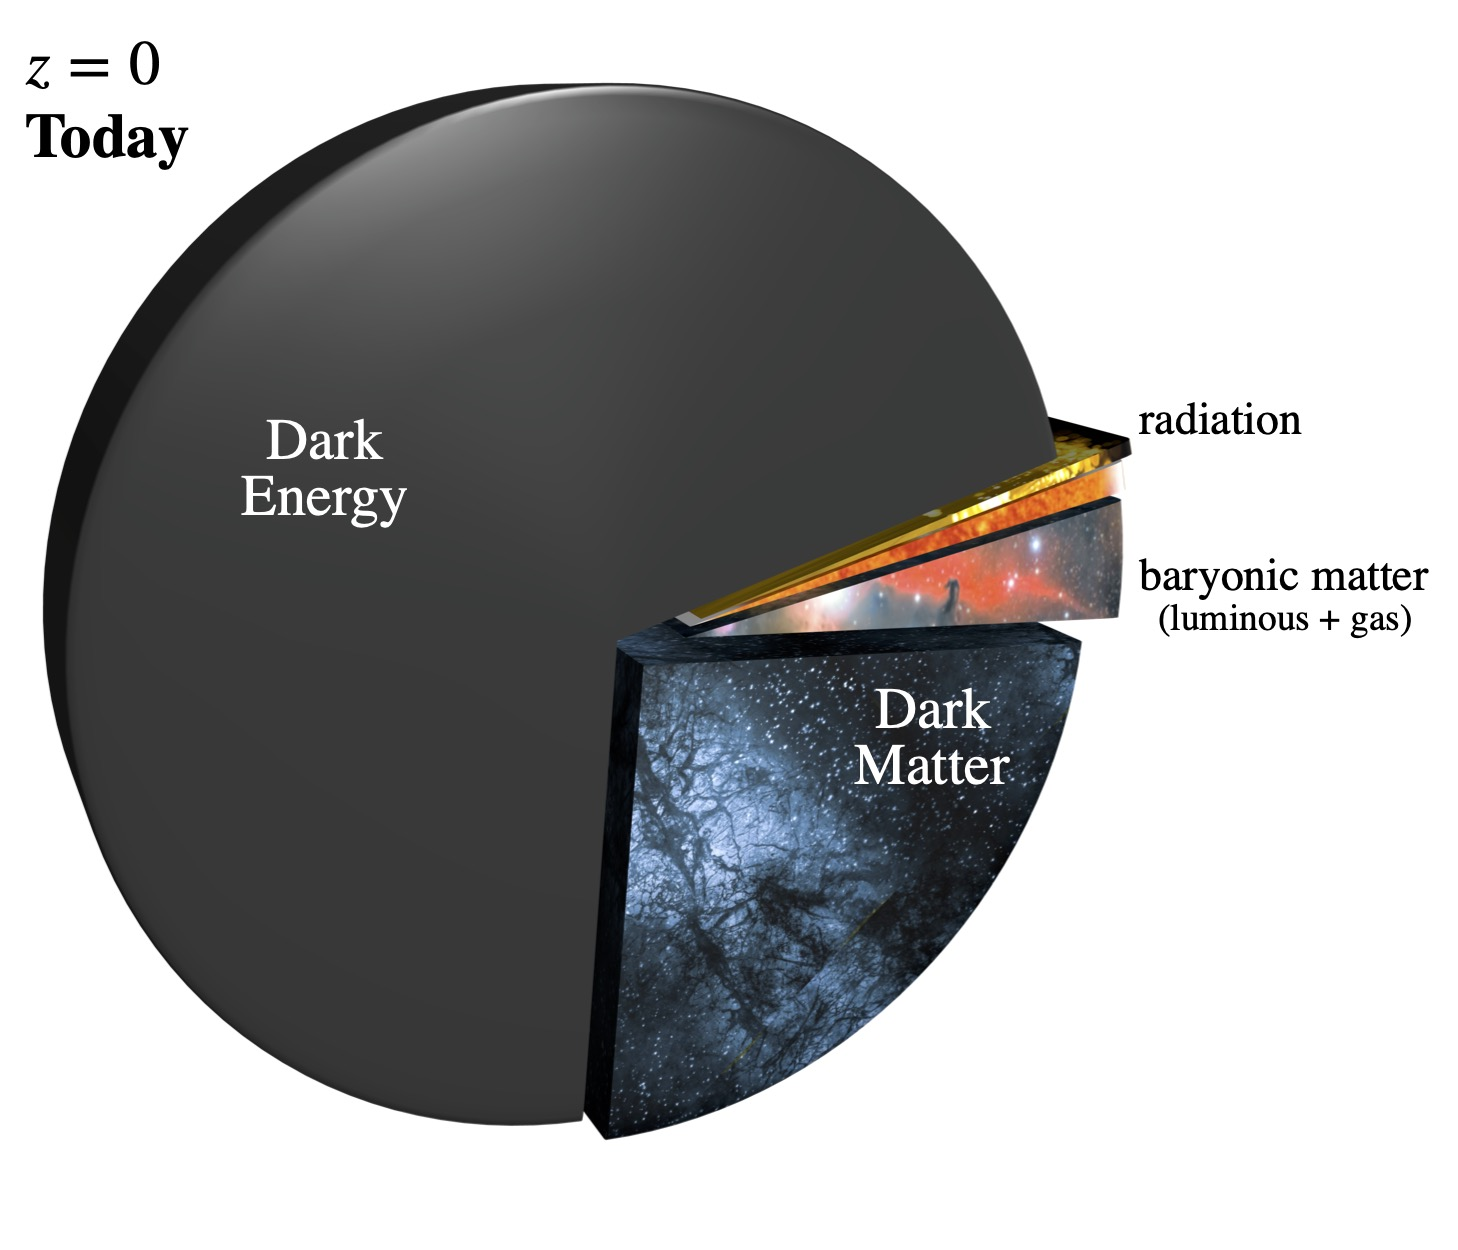
\includegraphics[width=0.47\textwidth]{figs/piechart1.jpg} \qquad
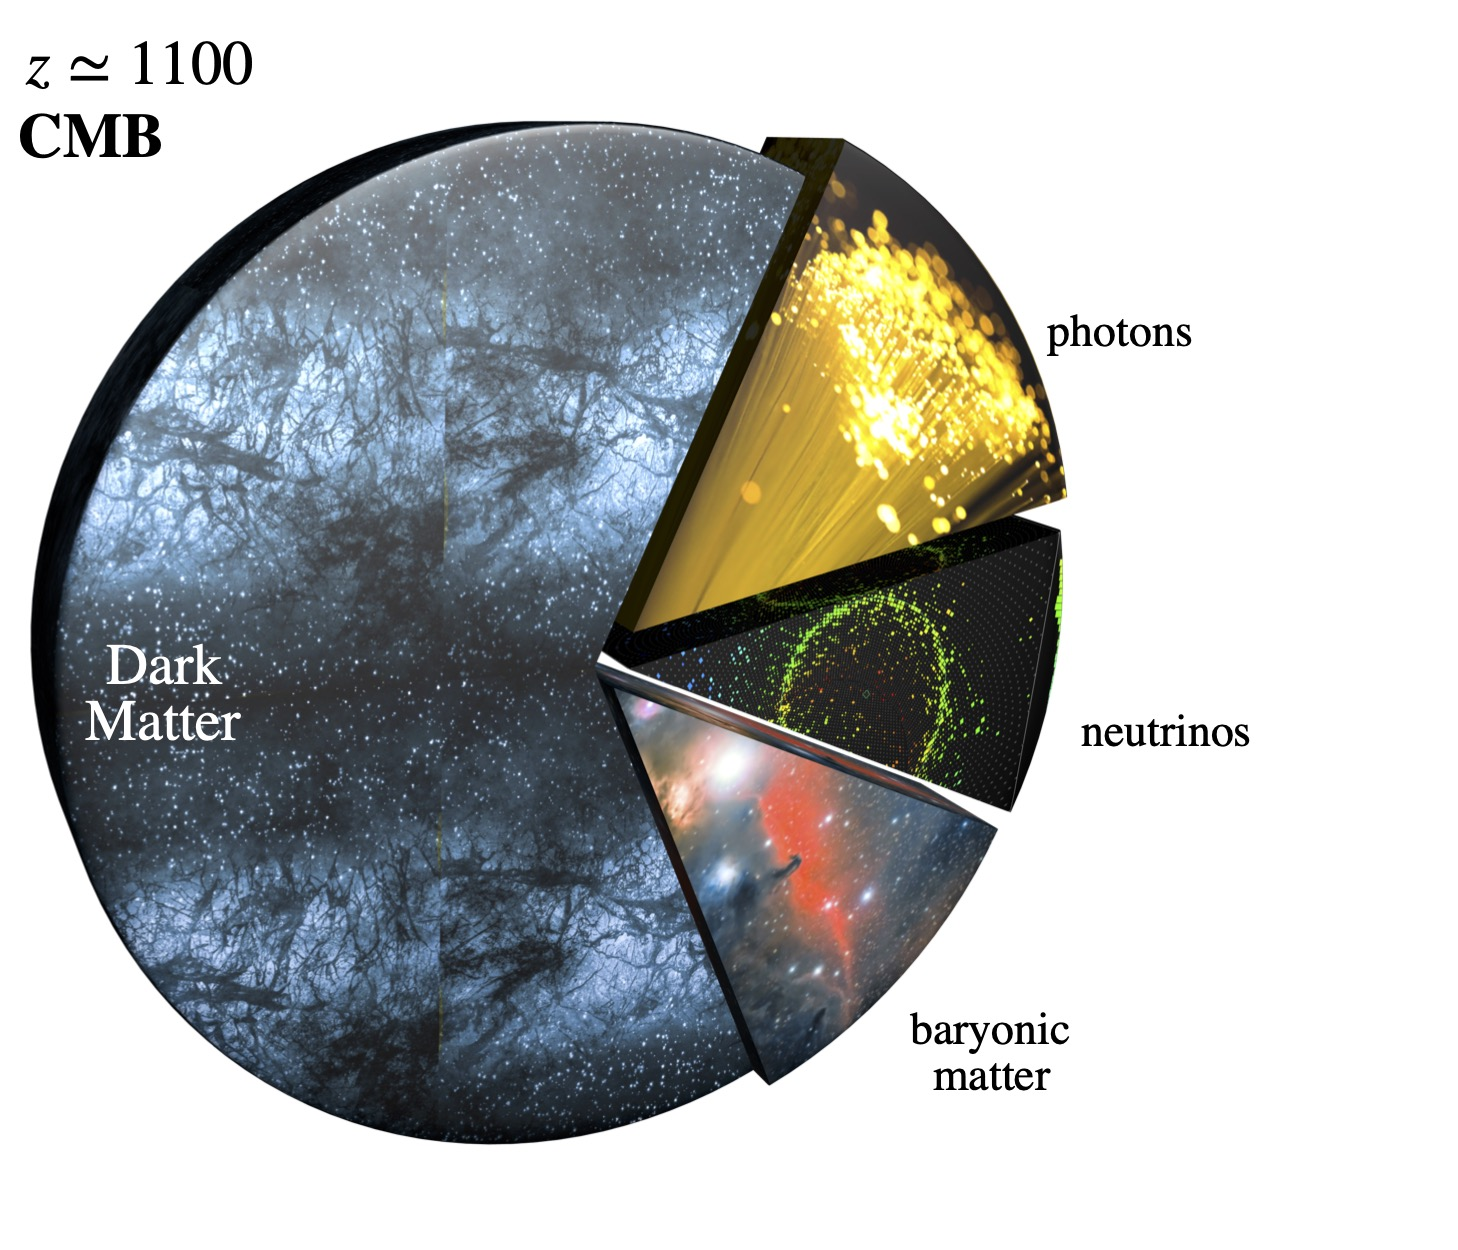
\includegraphics[width=0.47\textwidth]{figs/piechart2.jpg} \\[0.5cm]
\end{center}
\caption[Content of the Universe]{\em\label{fig:piecharts} {\bfseries Content of the Universe} today (left) and, for comparison, at the time of photon decoupling (right). The different components evolve differently in cosmology, see appendix~\ref{app:Cosmology}.}
\end{figure}


\bigskip

Next, let us summarize what the astrophysical and cosmological observations imply for the general properties of Dark Matter (in chapter \ref{paradigms} we will elaborate further for the specific cases, where DM is assumed to be made either of particles, fields or macroscopic bodies).
The data can be reproduced assuming that DM is a kind of {\em cold}, {\em non-interacting}, {\em stable matter}, with {\em adiabatic} inhomogeneities. 
\begin{itemize}
\item[$\circ$] {\bf Matter} stresses the fact that DM behaves as matter in the cosmological evolution, i.e., its density decreases as the inverse of the volume. In technical terms, its equation of state parameter is $w=0$ (see section \ref{sec:evidencesmaxi} and appendix \ref{app:matterenergy}). This is in contrast to Dark Energy, whose density, as far as we know, does not dilute in an appreciable way when the Universe expands.

\item[$\circ$] \index{Cold}\index{DM properties!cold}
{\bf Cold} means that DM behaves as a non-relativistic fluid at the crucial time of matter-radiation equality (MReq), when structure formation begins, and henceforth during all the subsequent periods of galaxy formation. The DM corpuscules move `slowly' and therefore attract each other and cluster. If they moved `fast', the clustering would not be effective and structures would not form and grow. The process of clustering does re-heat the DM fluid, since its constituents gain kinetic energy after collapsing into bound structures. However, this is not enough to make DM relativistic and invalidate the general coldness of DM, except perhaps in extreme environments, such as around compact bodies (see section \ref{sec:CaptureNS}). 
These points will be made more quantitative in section \ref{sec:linear:inhom} and chapter \ref{paradigms}.

\item[$\circ$] \index{DM properties!non-interacting}
{\bf Non-interacting} (or equivalently {\bf collision-less}) means that the interactions of DM with itself or between DM and ordinary matter (other than the gravitational interaction, which DM certainly possesses), are small enough to be neglected. This is what differentiates DM from ordinary matter. Whereas the latter has significant interactions, including in particular the electromagnetic one, DM does not. 
Therein lies the reason for the naming of Dark Matter --- the absence of interactions of DM with the light makes DM {\em dark}. 

This does not mean that DM absolutely can not have any interactions (other than the gravitational one) with itself or with the ordinary matter. Quite to the contrary, in most models the production of DM in the early universe does require non-zero interactions (as discussed at length in chapter \ref{chapter:production}). Furthermore, essentially all the search strategies rely on the existence of non-zero interactions  (see part \ref{part:detection} for details). Notably, DM particles with SM weak interactions, or with interactions of similar strength, fall into the `non-interacting' class, i.e., such interactions are feeble enough to be neglected in astrophysical considerations as well as for late cosmology.

\item[$\circ$]  A corollary of non-interacting is {\bf dissipation-less}: \label{dissipationless} unlike ordinary matter, DM cannot emit electromagnetic radiation and therefore cannot easily dissipate its energy and cool down. This feature is the core reason why ordinary matter and DM behave differently during the cosmological evolution. Of course, also in this case the prohibition is not absolute: interesting models exist in which DM has some small degrees of dissipation. 

\item[$\circ$] \index{DM properties!stable}
{\bf Stable} means that DM is present since the early phases of the Universe and has not disappeared until now (the current age of the universe being $t_{\rm Uni} \simeq 13.8 \ {\rm Gyr} = 4.35  \ 10^{17}$ s). Depending on the nature of DM, this will translate quantitatively into bounds on either the decay lifetime (if DM is made of unstable particles), or the evaporation rate (if DM is made of black holes subject to Hawking radiation), et cetera. See chapter \ref{paradigms}.

\item[$\circ$] \index{DM properties!adiabatic}
{\bf Adiabatic} means that, on cosmological scales,
the composition of the cosmological fluid is the same everywhere.
DM has the same primordial density inhomogeneity as the other components:
DM is denser where ordinary matter and photons are denser.
This happens if all the inhomogeneities have been generated by a single mechanism.
The mechanism is believed to be
quantum fluctuations of a single inflaton field during cosmological inflation.
Indeed, in agreement with this theory, 
all components seem to have a {\em Gaussian} and {\em quasi-scale invariant} spectrum of primordial fluctuations.
\end{itemize}




\section{Mini: galaxies}\label{sec:evidencesmini}

\subsection{Rotation curves of spiral galaxies}\label{sec:rotatiocurves}\index{Rotation curves}
Spiral galaxies\footnote{Traditionally, galaxies are classified according to their observed shapes as: Elliptical (E), Spiral (S) and Barred Spiral (SB). Elliptical galaxies are further labelled according to their elongation, from E0 (round) to E7 (very elongated). They do not exhibit any particular axis of rotation and are `dispersion supported' (as opposed to spirals and barred spirals which are `rotation supported'). Spiral and barred spiral galaxies are further delineated according to how tight their spiral arms wrap around the center: Sa, Sb, Sc\ldots and SBa, SBb, SBc\ldots, in order of increasing openness of the arms.  The Milky Way is a rather typical Sb galaxy. Irregular (Irr) and dwarf galaxies do not necessarily fall into one of the above classes. The classification does not necessarily correspond to an evolutionary scheme: generically, galaxies are not  born as E and then evolve to S or SB (although initially it was believed to be so) nor are they guaranteed to be created as S or SB and then merge into Ellipticals (although this is a recent hypothesis). This is currently an active research domain in astrophysics.}
rotate around their vertical axes. Measuring the Doppler shift of atomic lines one can determine the circular velocity of stars and other tracers (e.g.,~hydrogen clouds and masers) as a function of their distance from the galactic center, obtaining
a {\em rotation curve}. Some historical and recent examples are plotted in fig.~\ref{fig:rotationcurves}. 
Newton's law, $F=ma$, predicts a simple relation between the circular velocity $v_{\rm circ}$ of a test particle of mass $m$ (e.g.,~a star) and the mass ${\cal M}$ contained within a distance $r$ from the center, assuming spherical symmetry:
\beq\label{eq:vcirc}
m \frac{v_{\rm circ}^2(r)}{r} = \frac{G \, m {\cal M}(r)}{r^2} 
\qquad\Rightarrow\qquad
v_{\rm circ}(r) = \sqrt{\frac{G  {\cal M}(r)}{r}}.
\eeq
In spiral galaxies, most of the (visible) mass is concentrated in a dense central bulge and in the arms of the disk, which typically extend to $\mathcal{O}(10)$ kpcs. At large enough $r$, therefore, all the visible mass is contained within the orbit and can be replaced, in eq.~\eqref{eq:vcirc}, by a constant $ {\cal M}$.  
The velocity should then follow a Keplerian decline $v_{\rm circ}(r) \propto r^{-1/2}$.
The crucial point is that  the observations of a large sample of galaxies of this kind have shown that the rotation curves instead remain {\em flat} (i.e.,~constant in $r$) out to large distances from the galactic centers. Hence, according to
Newtonian gravity,
additional invisible mass must be present to prevent the peripheral stars from flying away and the galaxies from breaking apart. 

Assuming spherical symmetry, eq.~\eqref{eq:vcirc} shows that
a constant velocity $v_{\rm circ}(r)$ is obtained assuming a matter
 {\em halo} (containing a `dark' component) that has mass density $\rho(r) \propto 1/r^2$ out to large $r$: in this way, $ {\cal M}(r) = 4 \pi \int dr' \, r'^2 \rho(r') = 4 \pi \, r$ 
 so that the dependence of $v_{\rm circ}$ on $r$ vanishes. Eventually, at even larger $r$, the halo is expected to die off and the rotation curve to start declining. However, no tracers are typically available at such large distances.

\begin{figure}[!t]
\begin{center}
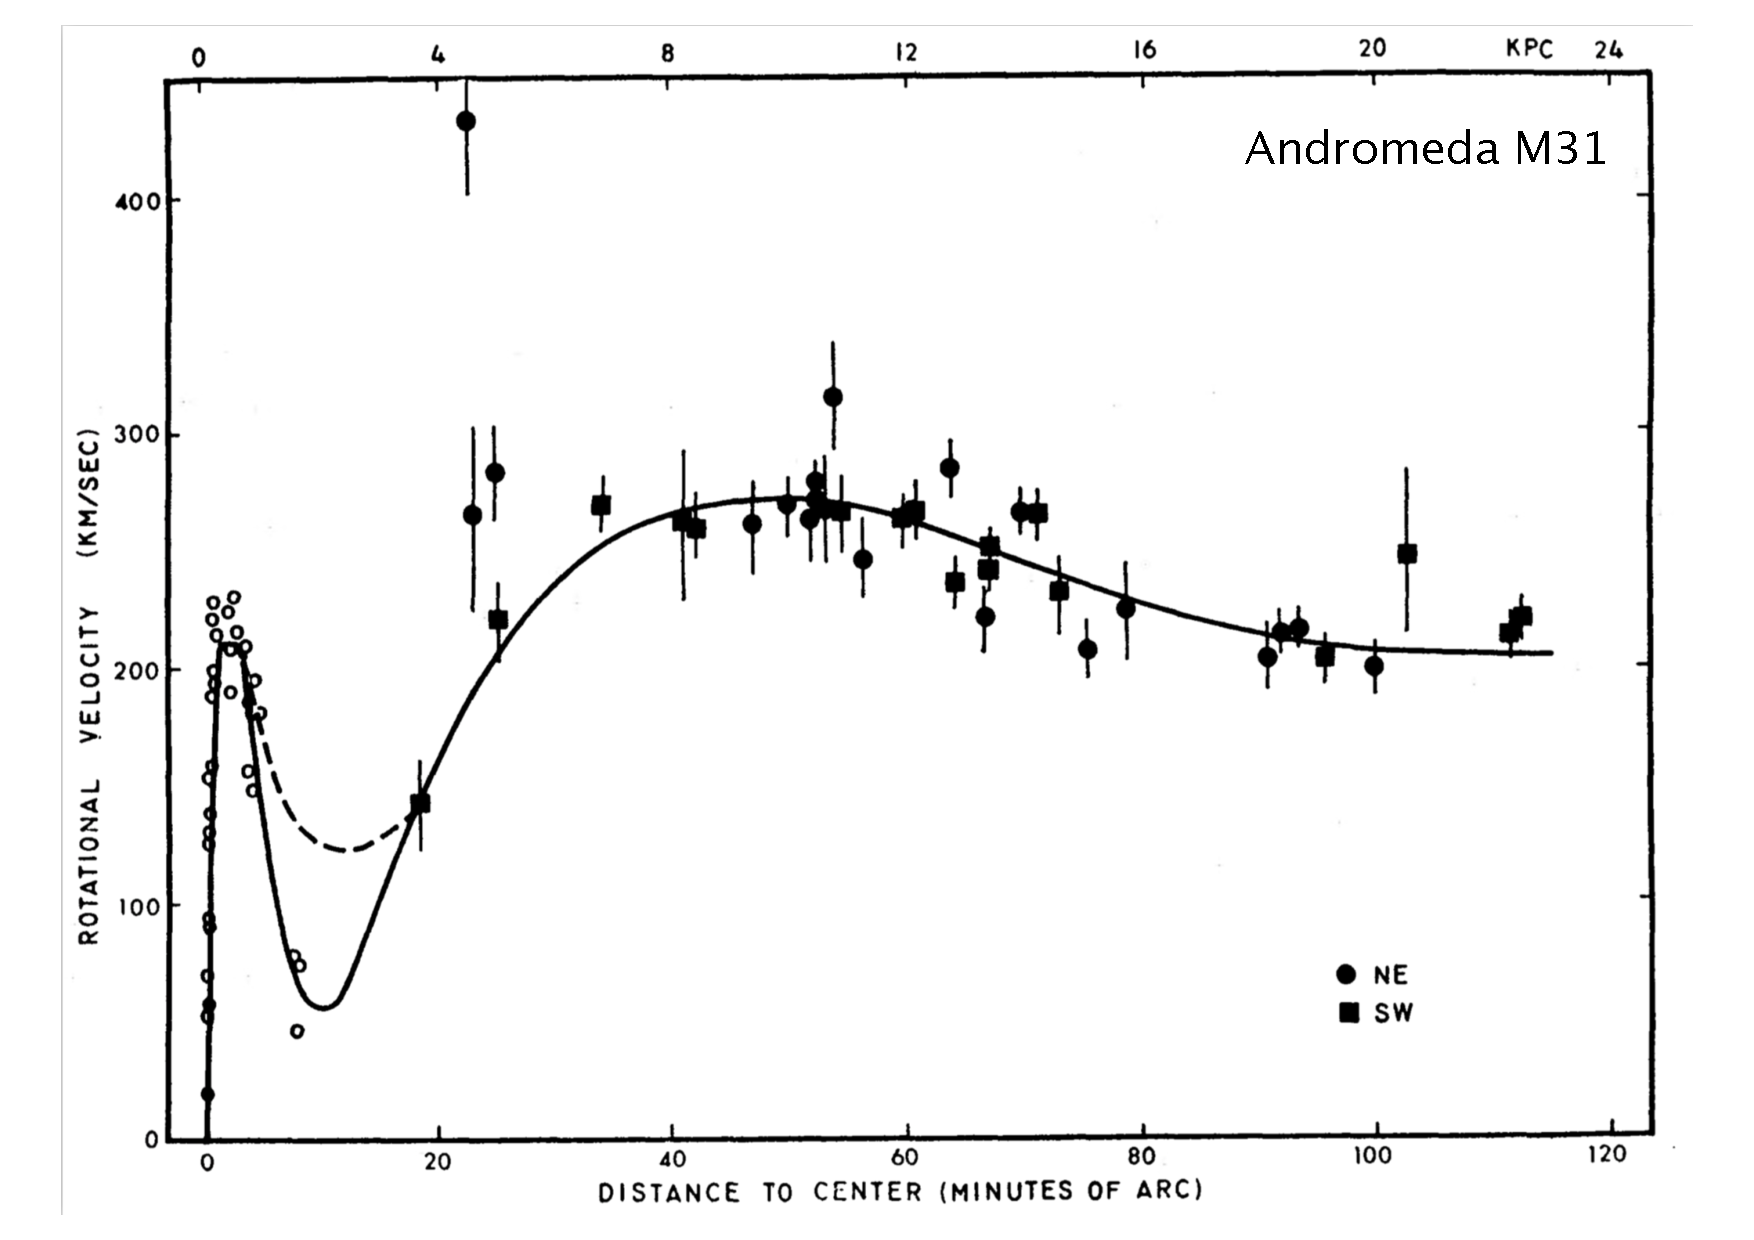
\includegraphics[width=0.45\textwidth,height=0.22\textheight]{figs/rotationcurve1_M31_RubinFord1970_mod}~
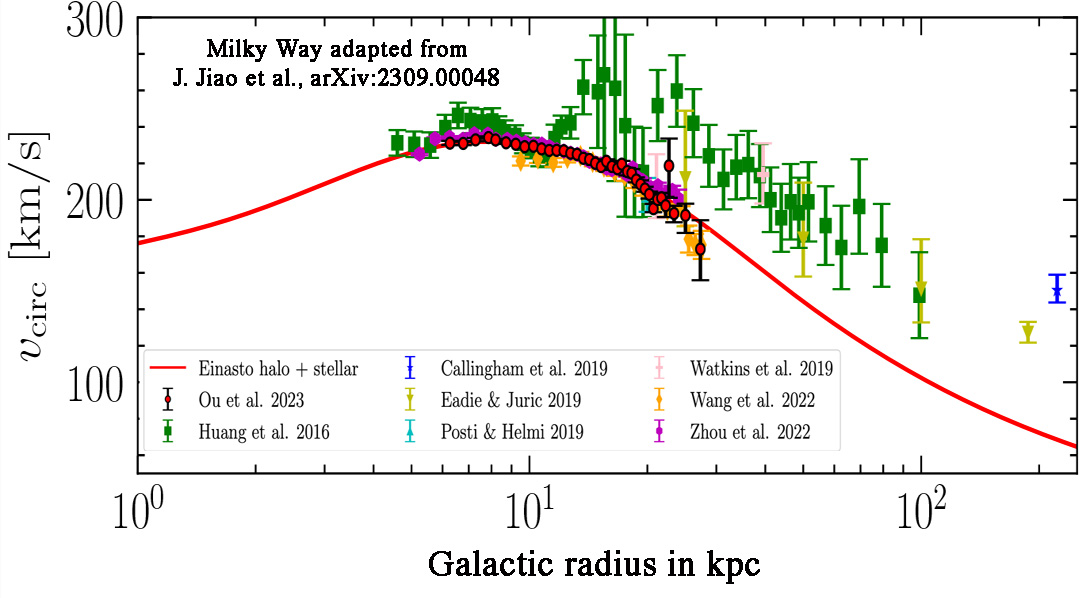
\includegraphics[width=0.45\textwidth,height=0.22\textheight]{figs/RotationCurveMW} 
\\[0.5cm]
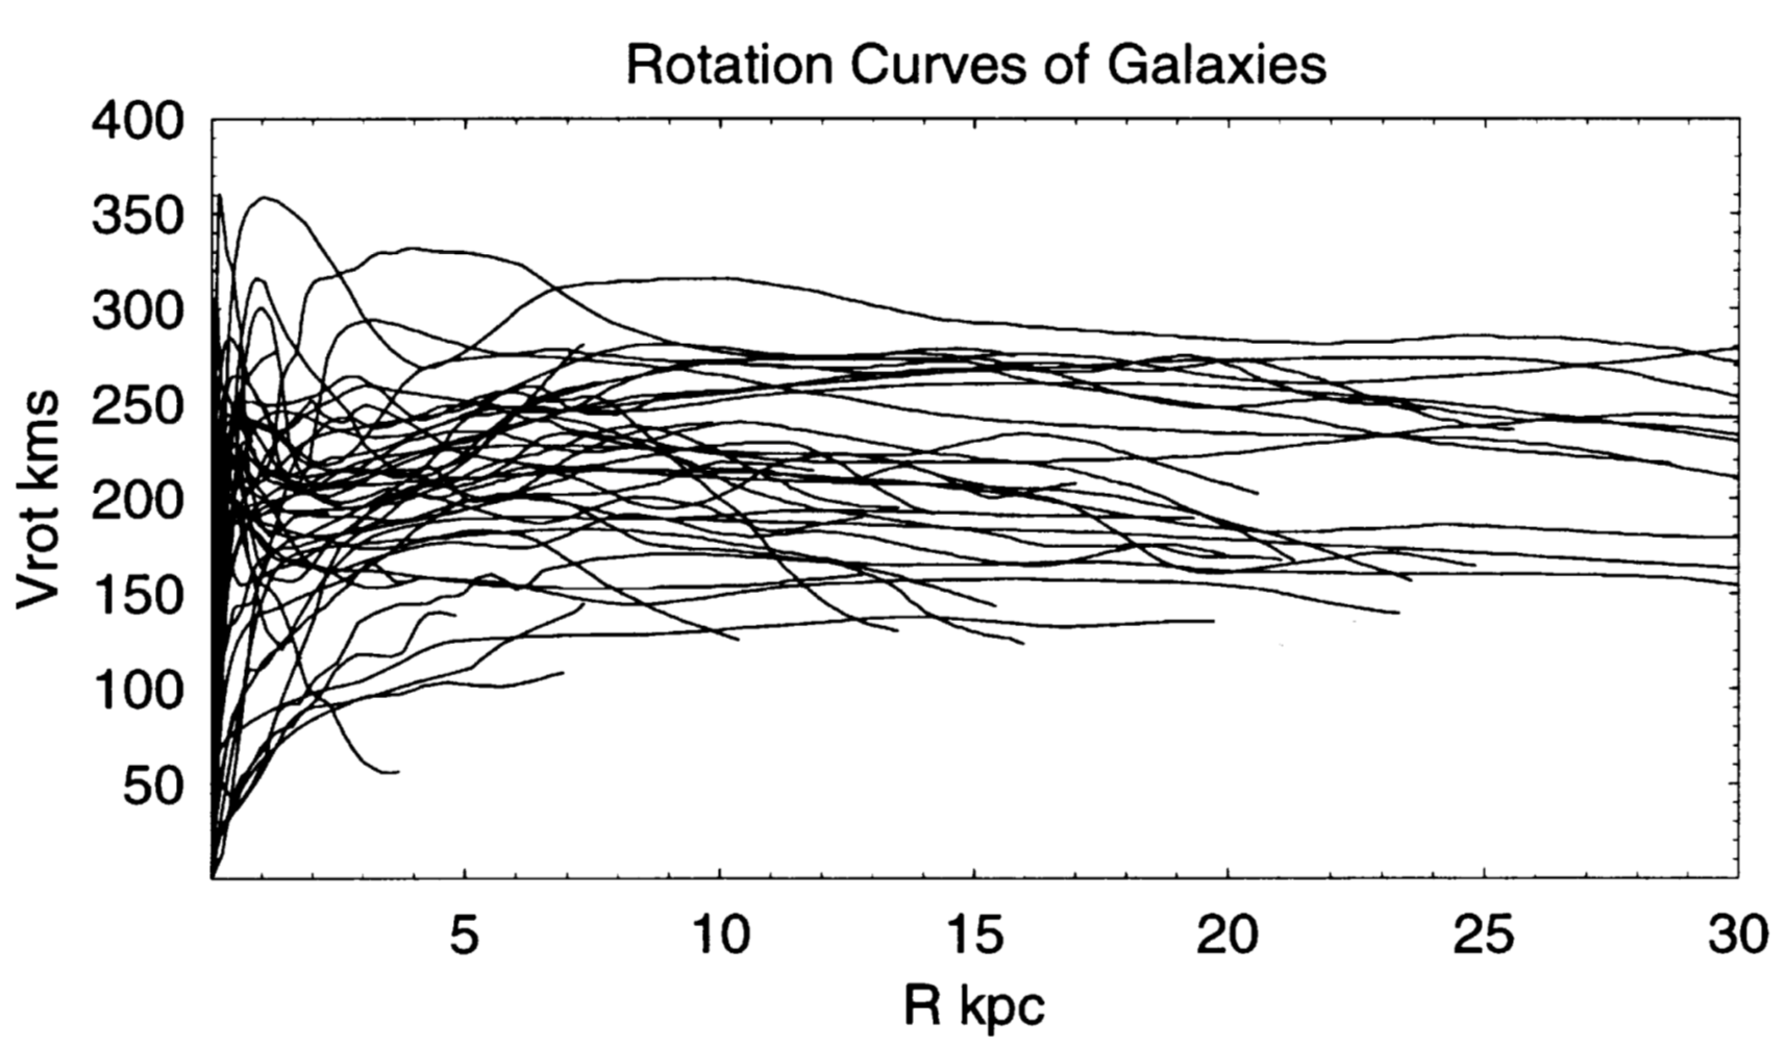
\includegraphics[width=0.45\textwidth,height=0.23\textheight]{figs/rotationcurve3_compilation_fromSofue1999.pdf}$\qquad$
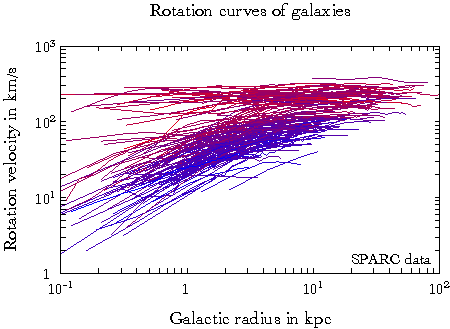
\includegraphics[width=0.44\textwidth]{figs/RotationCurveCompilationSPARC}~~
\end{center}
$$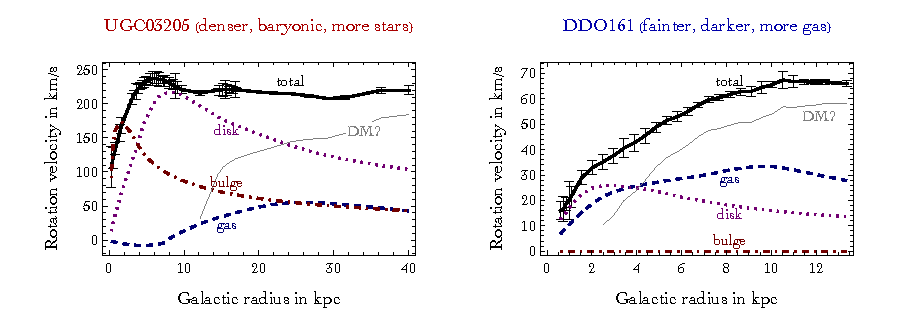
\includegraphics[width=0.97\textwidth]{figs/RotationCurveSample} $$
\caption[Rotation curves of spiral galaxies]{\em\label{fig:rotationcurves} {\bfseries Rotation curves of spiral galaxies~\cite{rotation_curves}}. 
{\bfseries Top left}: the original rotation curve of Andromeda by Rubin \& Ford (1970) ($\copyright$AAS, repr.~with permission). 
{\bfseries Top right}: a recent rotation curve for the Milky Way adapted from 
\arxivref{2309.00048}{Y. Jiao et al.~(2023)}~\cite{rotation_curves}, that shows a hint of Keplerian decline.
{\bfseries Center left}: a compilation of about 50 galaxies, from \arxivref{astro-ph/9905056}{Sofue et al.~(1999)} (repr.~with permission). 
{\bfseries Center right}: the \href{http://astroweb.cwru.edu/SPARC}{SPARC} compilation of 175 galaxies, 
from \arxivref{1606.09251}{Lelli et al.~(2016)}, color coded according to surface brightness
(red is denser, blue is fainter).
{\bfseries Bottom left}: a denser galaxy, dominated in its center by baryons, mostly in stars.
{\bfseries Bottom right}: a fainter galaxy, dominated by a dark component, with most baryons as gas.
The latter two plots show the total rotation velocity (black),
the contributions from disk stars (dotted magenta), in the bulge (dot-dashed red), from gas (dashed blue), and inferred DM (grey) from eq.~\eqref{eq:sum:v:squares}.
}
\end{figure}


\medskip 

Rubin and Ford~\cite{rotation_curves} performed in 1970 the first precise measurement of the rotation curve of the Andromeda galaxy (M31), tracing about 70 hydrogen clouds. They determined the curve to be rather flat out to $\sim22$ kpc.\footnote{Earlier observations do exist, notably by Babcock in 1939, Mayall in 1951 and Schwarzschild in 1954. While very interesting, they were, however, not as precise and/or did not extend as far in $r$, so that there was no consensus in their interpretations. For a detailed historical account see the review by \arxivref{1605.04909}{Bertone and Hooper (2016)} in~\cite{otherpastDMreviews}.} 
This was later corroborated by more observations, in tens of other galaxies and using radio as well as optical techniques, finding rotation curves that remain flat up to 50 kpc and beyond. 
The results were quickly interpreted as evidence for `missing mass' and the problem of Dark Matter rose to prominence. To this day, with hundreds of spiral galaxies observed, the flatness of rotation curves remains probably the most intuitive and convincing evidence in favor of DM. 

\smallskip

Realistic studies, as opposed to the simplified proof of principle sketched above, 
carefully model the different luminous components (bulge, bar, disk, gas\ldots) of the observed galaxies.
In astrophysical terms, it is said that they determine the proportion of invisible to visible mass, i.e.,~the `{\em mass-to-light ratio}', of a given galaxy. For a galaxy like the Milky Way or Andromeda, this ratio is of order 10. 
These measurements can also be used to determine the DM density profile, including in the Milky Way, although typically the result is not very constraining (see chapter~\ref{sec:rho_from_obs}). 




\subsection{Other galactic-scale evidences}\label{sec:othergalactic}
There are a number of  other pieces of evidence supporting the existence of DM that have been put forward, based on observations at galactic scales. 

First of all, the same kinematic measurements of tracers discussed in the previous subsection can be applied to other systems, in particular to {\it dwarf galaxies}. These are discussed in detail in section~\ref{sec:dwarfs}. The results show evidence for a large content of DM in these systems, with a mass-to-light ratio typically on the order of 100 or more.

\smallskip

Moreover, the determination of rotation curves of spiral galaxies can be performed using the dwarf galaxies themselves as tracers \cite{Zaritsky}. This approach corroborates the results obtained with other methods.

\smallskip

In the 1970s, early numerical simulations  and their analytical interpretations were showing that a dark spherical halo is needed to ensure 
the {\em stability of the disk} in spiral galaxies~\cite{disk_stability}. 
In its absence the simulated disks were seen to be disrupted within a few rotational periods and transformed into chaotic distributions of stars. 
Disruption was found  when the  rotational kinetic energy exceeds $\approx 14\%$ of the gravitation energy of the rotating disk.
In view of its geometry, a spherical DM halo increases the gravitational binding energy.
However, more sophisticated works  later showed that the DM halo also has the negative effect of morphing a disk into a bar and eventually 
slowing the rotation of the bar down, which is at odds with the observed existence of many spinning disks. 
Therefore, the role of dark matter in bar stability and disk dynamics appears to be complex and not easily summarized by a single conclusion.

\smallskip


The existence of massive DM halos around galaxies can also be proven via {\bf galaxy-galaxy lensing}~\cite{galaxy_galaxy_lensing}. 
This is the distortion of the images of background galaxies induced by the gravitational lensing effect of the foreground galaxies,
analogously to how the Sun gravitationally deflects the light of background stars. The deviation of the light trajectory is $\delta\theta=4GM_{\rm lens}/b$, where $b$ is the impact parameter and $M_{\rm lens}$ is the mass of the lens, in this case the foreground galaxy.
Geometric optics then implies that a lens with mass $M_{\rm lens}$ at distance $d_{\rm lens}$ gravitationally focuses a source object (at bigger distance $d_{\rm source}$)
into an `Einstein ring' (or arc) with angular size $\theta_{\rm E} = \sqrt{4GM_{\rm lens} (1/d_{\rm lens}-1/d_{\rm source})}$, if the source and the lens lie on the same line of sight, and into multiple images otherwise.
This phenomenon is known as {\em strong lensing}, despite the fact that the deviations are typically small, $\delta\theta\ll 1$, and is observable only when the lens is very massive, and the source close enough to it.
More commonly observed is {\em weak lensing}, where the lens is not strong enough to form multiple observable images or an arc, but does lead to a distorted image of the background galaxy.  
By measuring the average properties, as in fig.~\ref{fig:weaklensing},
one can infer the amount of matter in a typical lensing galaxy, finding that it is larger than the visible mass. 
The same observations can also determine the typical density profile of the DM halos, found to be somewhat flattened (see section~\ref{sec:asphericalcow}).  



 
 \subsection{DM-deficient galaxies?}\label{sec:DMdeficient}
In 2018  \arxivref{1803.10237}{van Dokkum et al.}~\cite{DMdeficient} claimed that the ultra-diffuse galaxy NGC1052-DF2 
(close to the giant elliptical NGC1052) 
contains little or no Dark Matter. 
Its stellar mass is evaluated at $2 \times 10^{8} \ M_\odot$, while its total mass is estimated, using the velocities of an unusual population of globular clusters as tracers, at less than a factor of 2 larger. This is a very surprising value for galaxies of this kind, which typically have a mass-to-light ratio of several hundreds. 
The results and the uncertainties have been closely scrutinised (e.g.,~whether the distance is really $\sim 20$ Mpc; if the galaxy is closer, then its inferred stellar mass would go down significantly and the mass-to-light ratio would increase). 
In 2019 the same group discovered NGC1052-DF4 in the same system, which had the same properties. 

The interpretation of these results, if they are confirmed, and their impact on the DM paradigm, have been debated. 
These galaxies could be explained away as just statistical outliers or as the result of a peculiar evolution that deprived them of their DM content (e.g.,~tidal stripping by a massive neighboring galaxy, or `bullet dwarf collision' events, similar in spirit to the bullet cluster discussed in section~\ref{sec:bullet}). 
In any case, it is fair to say that their existence poses a challenge to the standard theories of small galaxy formation. Some numerical simulations have not found any evidence of such galaxies in their results, while others have shown that small DM-deprived galaxies with the appropriate characteristics do form, thanks to close encounters with the massive host~\cite{DMdeficient}. 
Furthermore, these results would put stress on theories that use modifications of gravity rather than DM to explain rotation curves (see section \ref{sec:MONDproblems}), since in these theories one should always detect a modification of gravity in presence of ordinary matter, at large enough distances.




\section{Midi: clusters of galaxies}
\label{sec:evidencesmedi}\index{Galaxy clusters}
Fritz Zwicky is usually credited as having been the first person to lucidly claim the evidence for Dark Matter (`Dunkle Materie'), in 1933. 
However, as discussed by \arxivref{1605.04909}{G.~Bertone and D.~Hooper (2018)} in~\cite{otherpastDMreviews}, 
the concept and terminology of Dark Matter was already hovering in the astronomy community at the time, e.g.,~in the works by H.~Poincar\'e,  W. Thomson (a.k.a.~Lord Kelvin), E.~\"Opik,  J.~Kapteyn, K.~Lundmark and J.~Oort, as well as S.~Smith.
Zwicky's work is however historically important as well as particularly simple in retrospect, hence worth reviewing. 

By looking at the {\bf velocity dispersion in the Coma cluster of galaxies}, Zwicky found that extra matter was necessary to keep the galaxies together \cite{Zwicky:1933gu}. The clusters of galaxies are the largest gravitationally bound systems in the Universe. They contain hundreds to thousands of galaxies and extend to several Mpc in size (see fig.\fig{catalogue}). 
Because of their size, galaxy clusters are good probes of the `average' Universe. 
While the most precise determinations of average DM density at present do not come from galaxy clusters, they do lead to $\Omega_{\rm DM}\approx 0.2$. 

Zwicky's determination was based on the virial theorem. 
The virial theorem links the average kinetic energy to the average potential energy, $\langle K\rangle = -\frac{1}{2}\langle{V}\rangle$ for gravity.
In a toy system with $N\gg 1$ objects of mass $m$
at equal distance $r$ interacting through gravity, this allows to determine their total mass $mN$ from the velocity $v$ and the size $R$:
\beq  
\label{eq:Zwicky:toy}
N \frac{m v^2}{2} = \frac{1}{2} \frac{N^2}{2} \frac{Gm^2}{R}
\qquad\Rightarrow\qquad
mN=\frac{2Rv^2}{G}.
\eeq
Applying such considerations to the Coma cluster of galaxies,\footnote{Zwicky approximated the cluster with a different toy model than in eq.~\eqref{eq:Zwicky:toy}: a sphere of constant density $\rho$ and radius $R$. The results differ by order one factors, with the average potential energy now given by $-\langle{V}\rangle = \int_0^R G \, \rho \, 4\pi r^2 dr M(r)/r = 3 GM^2/5R$, where $M(r)$ is the mass enclosed in $r$ and $M$ is the total mass.} 
Zwicky argued that the total mass in the cluster was larger than the visible mass, such that extra dark matter was needed.\footnote{Nowadays we measure that, in a typical cluster, the mass of the stars in galaxies represents $1-2\%$ of the total mass and the intergalactic gas represents $5-15\%$. The rest is missing and is interpreted as DM~\cite{bulletcluster}.}  The DM hypothesis was not widely accepted, but it was also not disregarded.  A common interpretation was that more information would be needed in order to understand these systems. 

\medskip

Since the 1980s, {\bf $X$-ray observations} have emerged as a more effective method for assessing the amount of ordinary and dark matter within galaxy clusters 
(for reviews see~\cite{Xrayclusters}). 
Galaxy clusters contain large amounts of ionized hydrogen and helium. 
When this gas collapses into the cluster's potential well, it undergoes shocks and adiabatic compression, heats up, 
and reaches temperatures  $T_{\rm gas} \sim m_p v_{\rm esc}^2 \sim 10\keV\sim 10^8\,{\rm K}$, which would be typical of nuclear reactions.
However, due to the low ambient density, nuclear fusion is negligible.
The gas then emits $X$-rays, primarily through thermal bremsstrahlung. 
Assuming spherical symmetry and hydrostatic equilibrium, one can write down the equilibrium equation
which links the gradient of the gas pressure, $\wp_{\rm gas}$, to the gradient of the gravitational potential, $\phi$,
\beq
\label{eq:hydrostaticcluster}
\frac{1}{\rho_{\rm gas}(r)}\frac{d\wp_{\rm gas}}{dr} = - \frac{d\phi}{dr} = - \frac{G M(r)}{r^2},
\eeq
where $\rho_{\rm gas}(r)$ is the gas density and $M(r)$ the total gravitating mass (i.e., hydrogen/helium gas and dark matter) within radius $r$. Assuming an ideal gas, the pressure and density are related via $\wp_{\rm gas} = \rho_{\rm gas} k T_{\rm gas}/\mu m_p$, where $\mu \approx 0.6$ is the mean molecular weight of an admixture of $\sim75\%$ hydrogen and $\sim25\%$ helium. The density $\rho_{\rm gas}$ and the temperature $T_{\rm gas}$ can be measured from the intensity and the spectrum of the $X$-ray emission, thereby allowing to reconstruct the total cluster mass as well as its profile using eq.~(\ref{eq:hydrostaticcluster}). The results confirm that the gas constitutes only a portion of the total mass of the galaxy cluster.
In a way, the use of $X$-ray emissions is an application of Zwicky's method to the microscopic scale:
 the kinetic energy  of the gas molecules (i.e., their temperature) takes the place of that of the galaxies, from which one then infers the total gravitating mass that keeps the galaxy cluster gravitationally bound. 

$X$-ray measurements also prove very useful in a different way, namely in analyzing unique spatial configurations such as the collisions of galaxy clusters, which we discuss next.




\subsection{Weak gravitational lensing: the bullet cluster and cosmic shear}
\label{sec:bullet}\index{Weak lensing}\index{Bullet cluster}

\begin{figure}[t]
\begin{center}
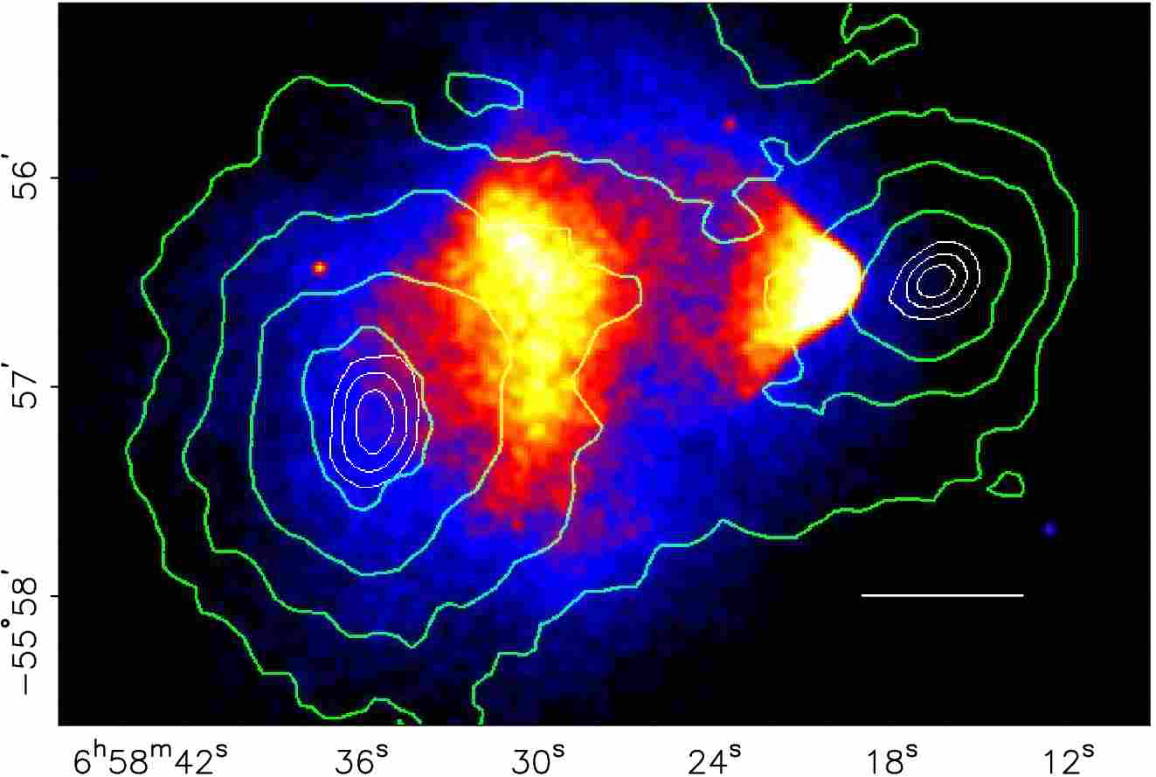
\includegraphics[width=0.6\textwidth]{figs/f1b_new_jpeg2ps}
\end{center}
\caption[Bullet cluster]{\em\label{fig:bullet:cluster} {\bfseries Bullet cluster}. 
The collision of a pair of clusters of galaxies, with the colored map representing the X-ray image of the hot baryonic gas. This is displaced from the distribution of the total mass reconstructed through weak lensing, shown with green contours. The white bar corresponds to the length of $200 \kpc$. 
From \arxivref{astro-ph/0608407}{Clowe et al.~(2006)} in~\cite{bulletcluster} ($\copyright$AAS, reproduced with permission).}
\end{figure}


Today, one of the most striking evidences for the presence of DM on the length scales of galaxy clusters comes from the 
observations of a pair of colliding clusters known as the {\em bullet cluster} located 3.7 Gyr away,
with a catalog name 1E0657-558 (or 1E0657-56) and first observed in detail in 2006, as well as from similar systems~\cite{bulletcluster}. 
Most of the baryonic mass in the bullet cluster is in the form of hot gas whose distribution can be traced through its $X$-ray emissions. 
The distribution of the total mass, visible and dark, was independently measured through weak lensing. 

The special feature of the bullet cluster system is that the visible matter and Dark Matter are spatially separated, see fig.~\ref{fig:bullet:cluster}.
The interpretation is the following: in the past, each of the two clusters of galaxies was an ordinary system,
with the visible matter and DM mixed together.
The two objects collided 150 million years ago.
Visible matter interacts significantly with itself, so that the hot gas from the two clusters experienced a collisional shock wave.
DM, on the other hand, experienced negligible collisions with itself and with normal matter, such that 
the DM clouds of the two systems simply passed through each other.
This led to the present separation of the visible and dark matter components, apparent in fig.~\ref{fig:bullet:cluster}.\footnote{Detailed studies reconstruct an initial relative velocity of about 3000 km/s before the collision between the two clusters. This had been claimed to be unusually high: according to the tails of velocity distributions in $\Lambda$CDM cosmology, the probability of observing such an event had been claimed to be too low ($\sim 10^{-5}$ assuming a reasonable amount of matter inhomogeneities)~\cite{BulletClustervelocity}. Hence the bullet cluster, in this specific aspect of the relative speed, had been used as evidence {\em against} Dark Matter. Later studies, however, have disputed the claim and found probabilities that are in agreement with $\Lambda$CDM cosmology~\cite{BulletClustervelocity}.}
After the observation of the bullet cluster, many similar systems have been studied. 
\arxivref{1503.07675}{Harvey et al.~(2015)}~\cite{bulletcluster} report the results on 72 of them and conclude that the existence of DM can be established with a significance of more than 7$\sigma$.


This kind of observations puts a severe strain on alternative interpretations where DM is replaced by a modification of gravity.  
Such modifications cannot get spatially separated from normal matter (unless they too introduce something that effectively behaves as DM),
so that the anomalous lensing signal would follow the distribution of the visible matter, as we will discuss in more detail in chapter~\ref{sec:MOND}.

\medskip

The bullet cluster and similar systems also provide information about the particle physics properties of DM. The fact that the DM halos did not slow down compared to the collision-less trajectories implies an upper bound 
 $\wp \sim \sigma \, n \, r_{\rm cl} \circa{<}1$ 
on the probability $\wp$ that a DM particle scatters with another DM particle on the typical scale of the system.
Here $\sigma$ is the DM self-interaction cross section, 
$n$ the DM number density and $r_{\rm cl}$ the size of the cluster.
In the specific case of the bullet cluster, data indicate  $r_{\rm cl} \sim 150$ kpc
and $\rho \sim 0.5 \, {\rm GeV/cm}^3$.
Observations provide information on the DM density $\rho = M n$ (and not directly on the DM number density $n$), 
so one obtains a bound on $\sigma/M$, where $M$ is the DM mass.
Different studies find slightly different values~\cite{bulletcluster,selfinteractionlimits}, 
in the ballpark  of (within roughly a factor of 2)
\beq \label{eq:bulletbound}
\frac{\sigma}{M}\lesssim 1\, \frac{{\rm cm}^2}{{\rm g}}= \frac{1.8 \,{\rm mb}}{\GeV}=
\frac{4580}{\GeV^3},
\eeq 
when assuming point interactions.\footnote{The baryonic gas, on the contrary, has long-range (Coulomb) interactions, whose effective cross-section is much higher that the limit: the typical atomic cross section corresponds to the Bohr radius squared $\sigma \sim 1/(\alpha m_e)^2 \approx 10^{-20} \, {\rm m}^2$, hence $\sigma/M \sim 10^8 \, {\rm cm}^2/{\rm g}$.} For comparison, 50 mb is a typical QCD cross section, for, e.g.\ $pp$ scattering.
The bound in eq.~\eqref{eq:bulletbound} is thus satisfied if DM is made of particles somewhat heavier than protons and/or somewhat less strongly interacting than protons.
The DM/matter cross section is similarly bound by astrophysics and cosmology to be roughly smaller than QCD size at $M\sim 1$ GeV, although a number of other much more stringent constraints apply (see the full discussion in section~\ref{sec:SIMP}).



\medskip

\begin{figure}[!t]
\begin{center}
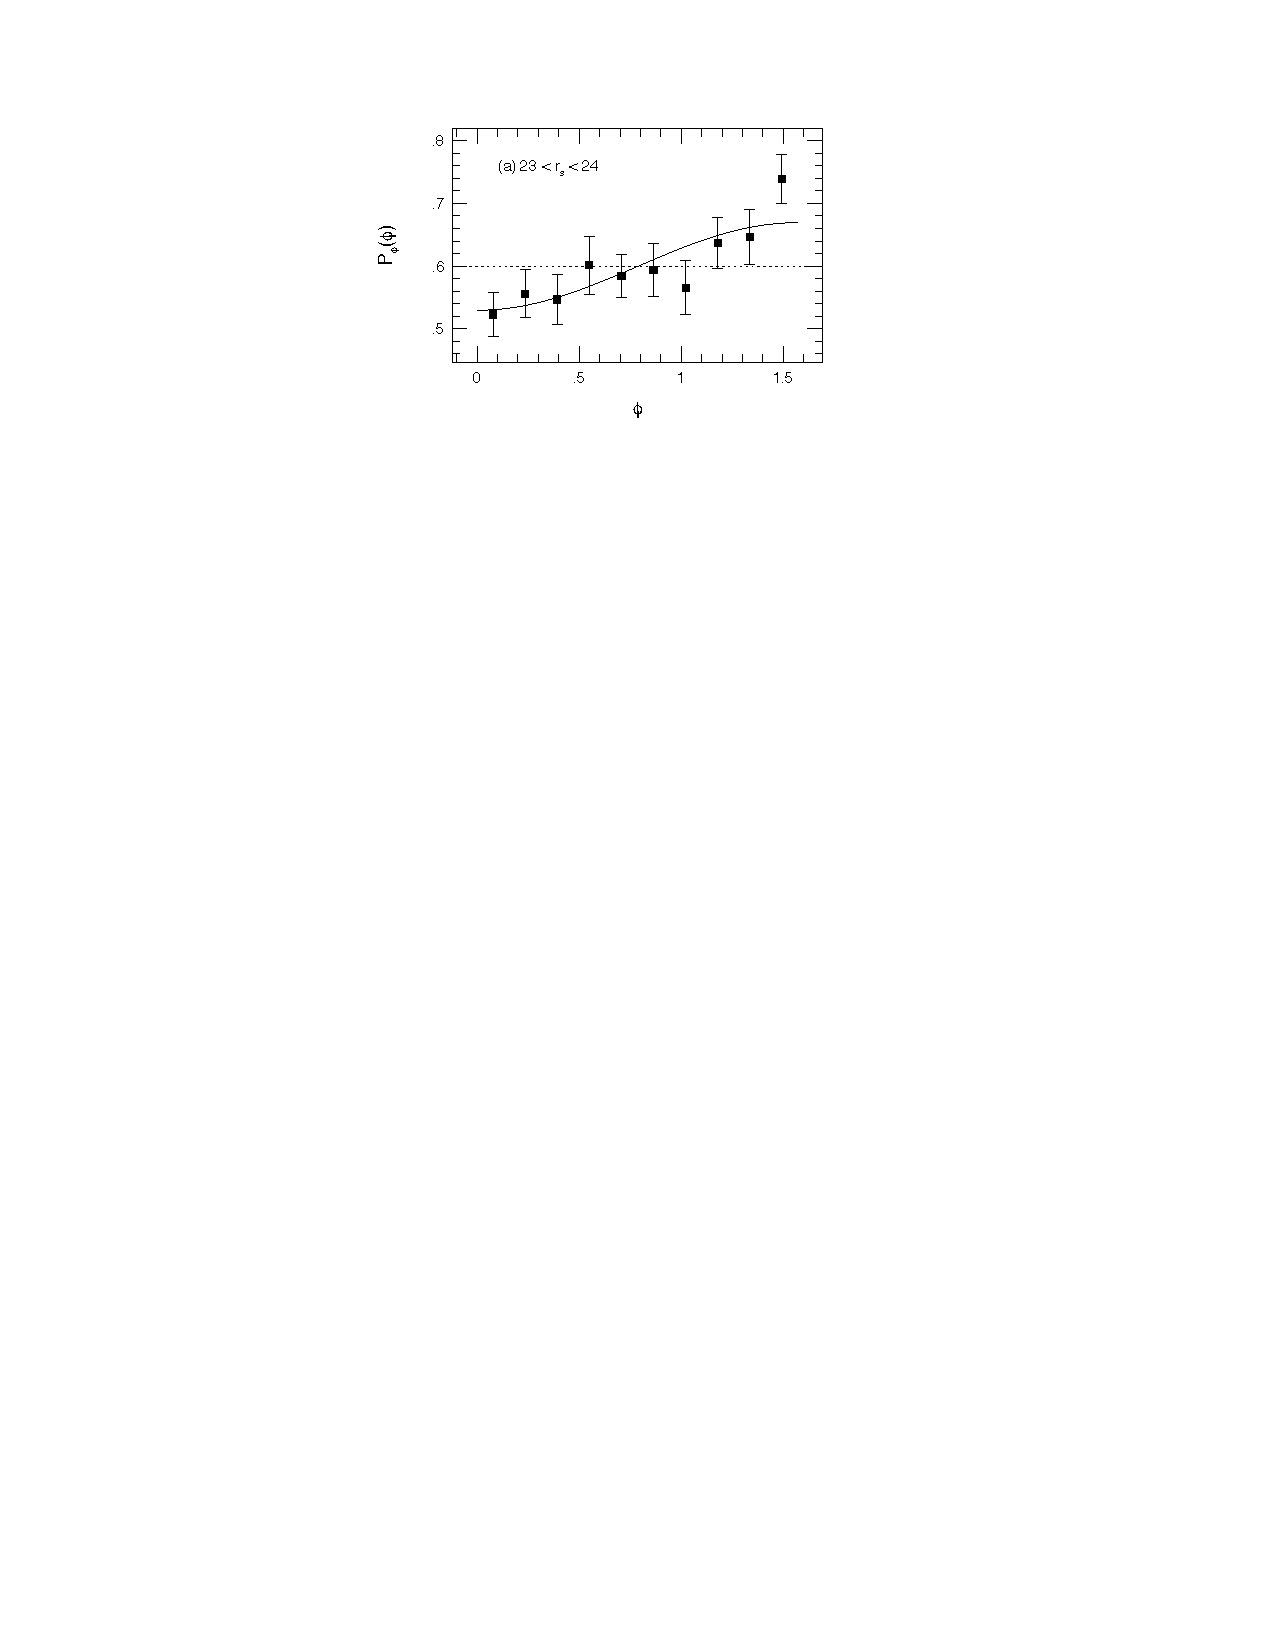
\includegraphics[width=0.46\textwidth,height=0.32\textwidth]{figs/galaxygalaxylensing_Brainerd1995.pdf} \qquad
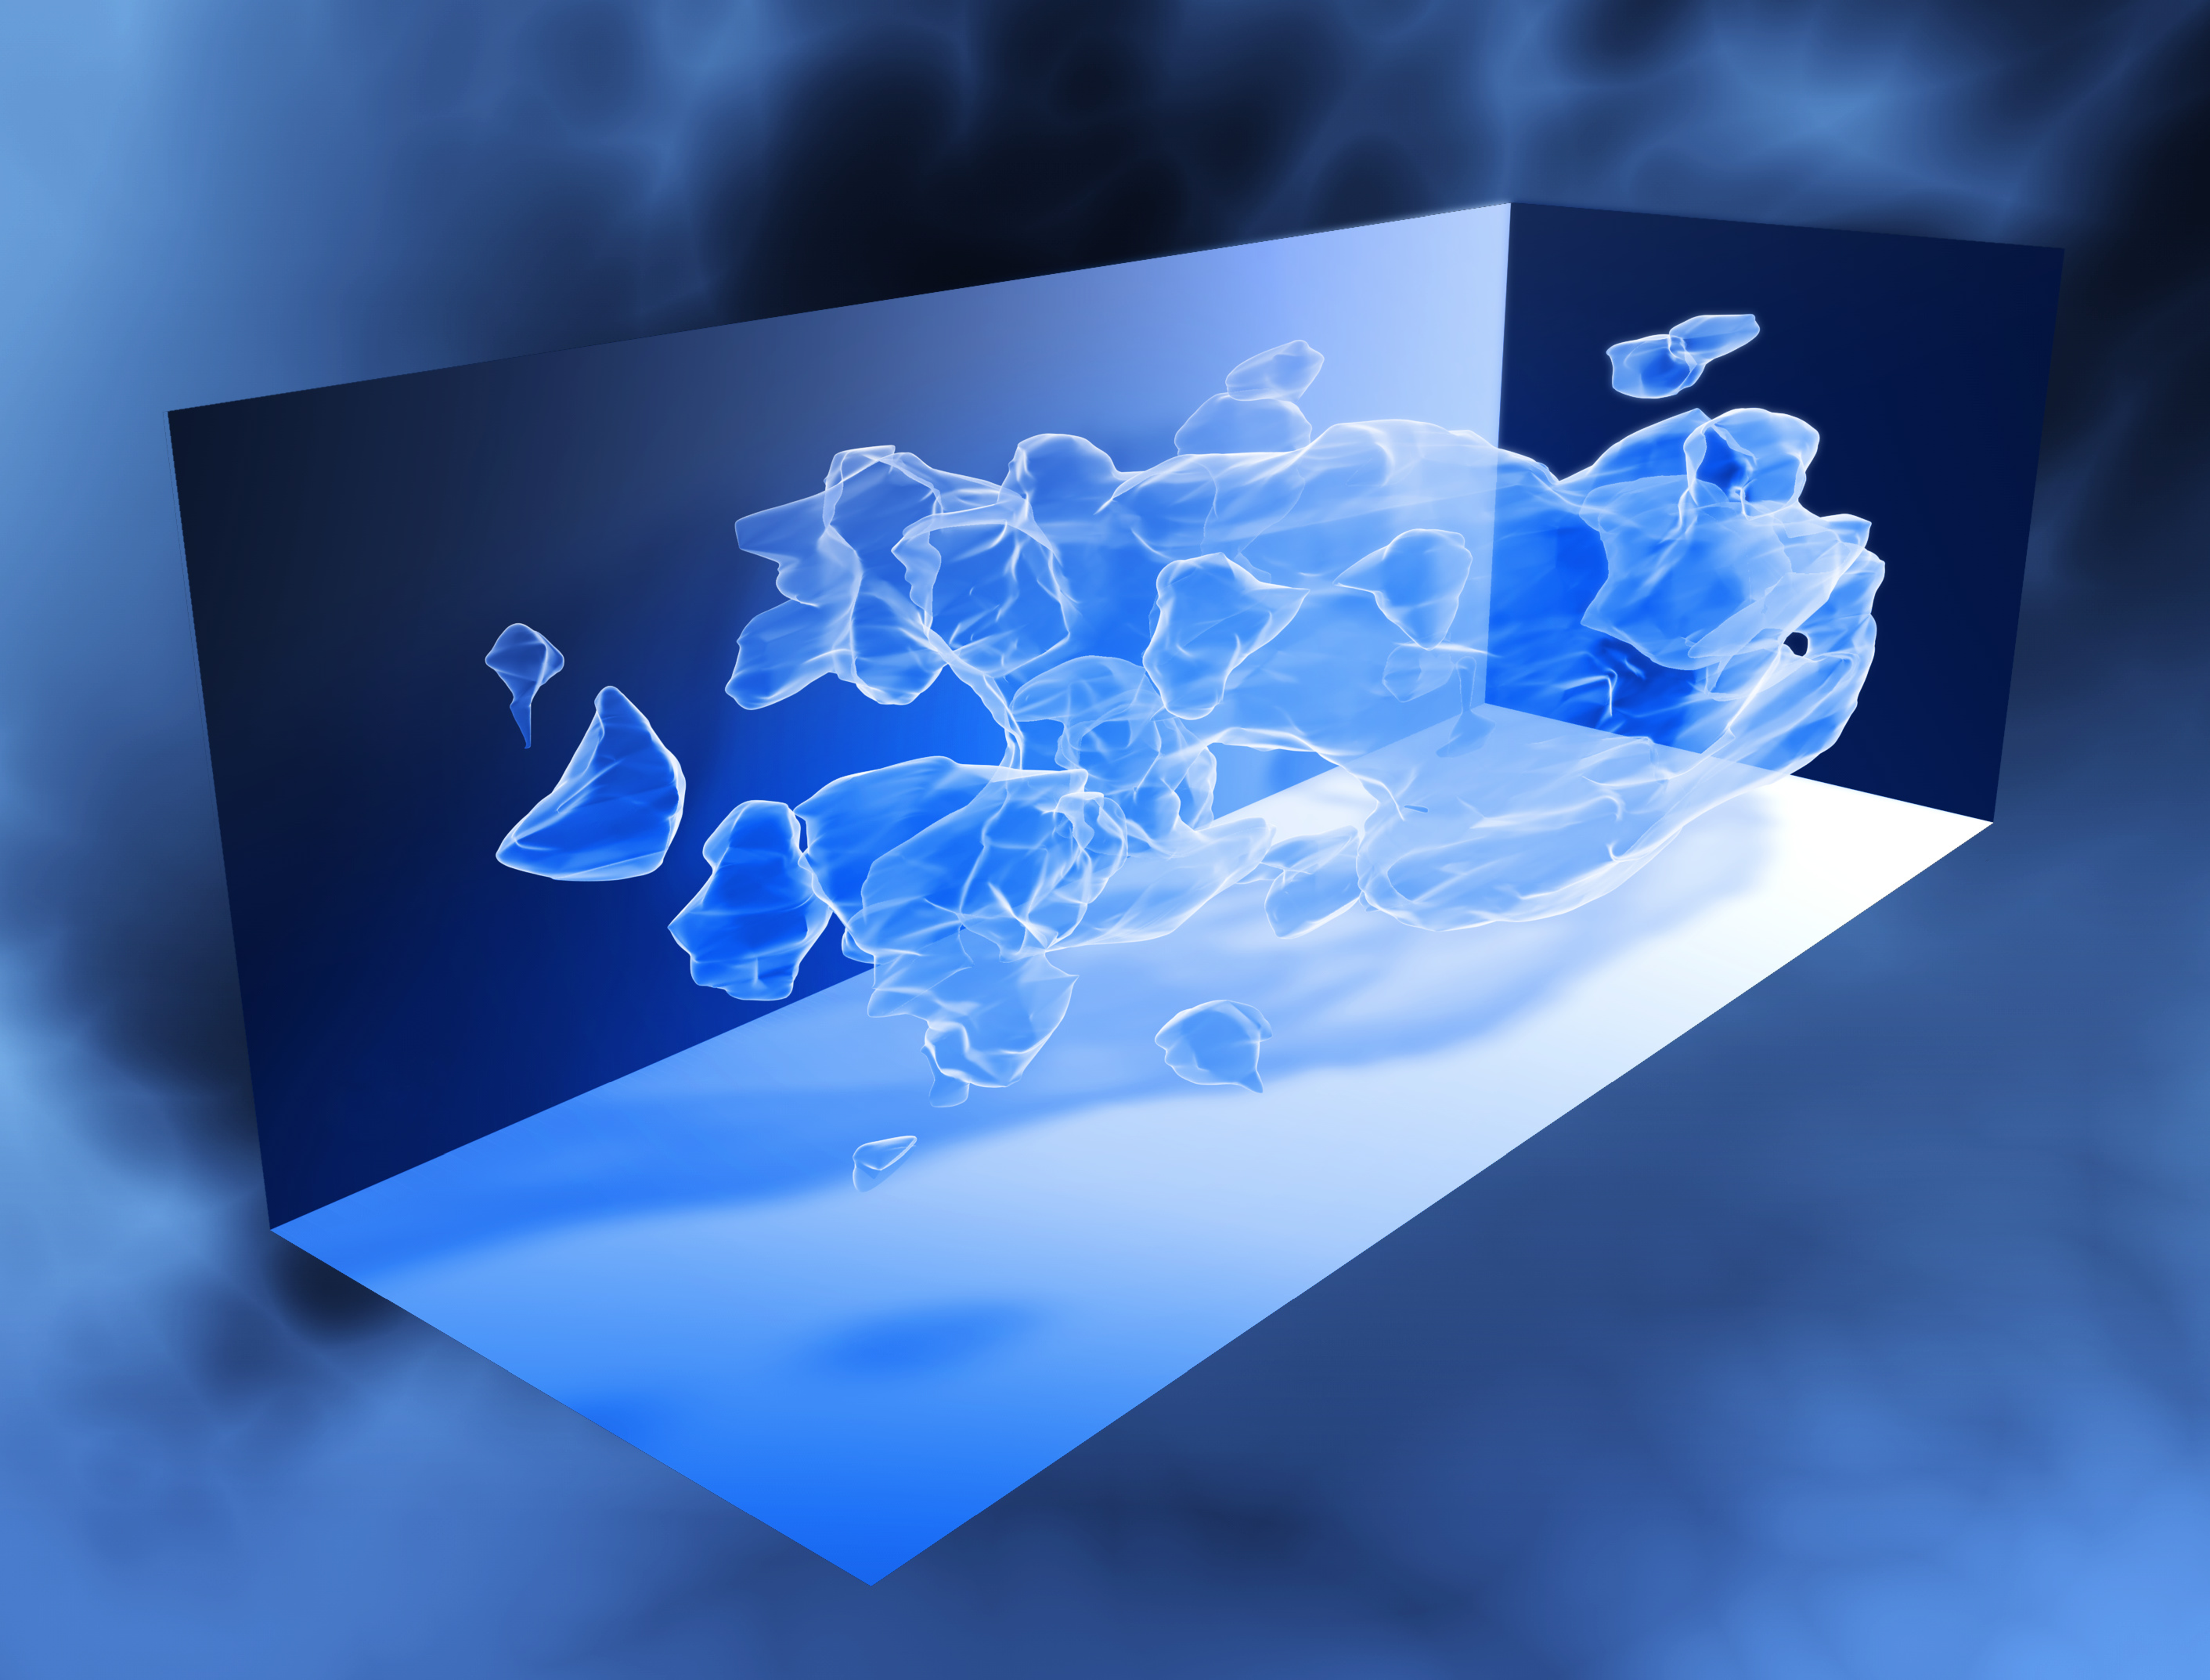
\includegraphics[width=0.46\textwidth,height=0.32\textwidth]{figs/cosmicshear_MasseyNature2007_alternative.pdf}
%\includegraphics[width=0.46\textwidth,height=0.32\textwidth]{figs/cosmicshear_MasseyNature2007.pdf}
\end{center}
\caption[Weak lensing]{\em\label{fig:weaklensing} {\bfseries Weak gravitational lensing} is a multi-length and multi-purpose tool to establish the existence of Dark Matter and determine its properties. 
At small scales the important effect is galaxy-galaxy lensing (discussed in section~\ref{sec:othergalactic}), see the left panel. 
The images of background galaxies are statistically distorted to align on a ring pattern around a foreground galaxy. That is, for a certain bin in magnitudes ($r_s$) of the source galaxies, the average probability of the orientation is measured to have a deficit of images oriented radially ($\phi = 0$) and an excess of images oriented tangentially ($\phi = \pi/2$). 
At very large scales the important effect is cosmic shear (section~\ref{sec:bullet}), see the right panel. The clouds in the graph are the constant density contours of the large scale DM formations, as reconstructed in 3D by the observations of the lensing of background sources. (Figures from Brainerd et al.~1995 in \cite{galaxy_galaxy_lensing} ($\copyright$AAS, reproduced with permission), credit: NASA/ESA/Richard Massey).}
\end{figure}


\medskip


\subsubsection{Cosmic shear}\index{Cosmic shear}
At length scales somewhat intermediate between the galactic/cluster and the cosmic scales, 
the detection of {\em cosmic shear} also provides evidence for DM~\cite{cosmicshear}. Cosmic shear refers to the deflection of light from very distant galaxies by the gravitational attraction due to the foreground mass concentrations. These are not in the form of the DM halos of galaxies or clusters (as was the case for the galaxy-galaxy lensing and for the case of cluster collisions, discussed above), but rather in the form of much larger and diffuse structures such as vast filaments and loose clumps. The measurements are performed statistically on a very large number (millions) of distant galaxies using multi-wavelength surveys, which have to be 
very deep (detecting very distant galaxies) and very wide (exploring large portions of the sky). 
The shapes of distant galaxies are distorted by the shear, changing the major-to-minor axis ratios by about $ 2\%$, which can be detected on a statistical basis. 
The observations determine $\Omega_{\rm DM}\approx 0.25$. 

The importance of cosmic shear goes well beyond the mere additional evidence for the existence of DM. By reconstructing the matter distribution along the line of sight, one is effectively looking back at the formation history of the large DM structures that provide the scaffolding of the Universe, which we discuss in the next section.

\smallskip
A phenomenon along similar lines is the so called {\bf CMB lensing}, which involves searching 
 for distortions of the CMB map caused by the foreground mass concentrations. 
In a way, this is the ultimate application of weak gravitational lensing as a tool to  probe DM. Since the CMB is the earliest observable light, it provides a unique opportunity to investigate the extremely large DM structures at high redshifts ($z \gtrsim 2$). CMB lensing has been detected with high statistical significance, both in data from {\sc Planck} as well as from other experiments (see \cite{CMBlensing} for a review and recent {\sc Planck} results), corroborating the evidence for DM.
The effect of lensing is to reshuffle the CMB perturbations. Notably, it smooths out the peaks at large $\ell$ in the CMB power spectrum and affects the polarization of the CMB photons, creating the so called $B$ modes out of $E$ modes. In fact, from the perspective of someone interested in the primary CMB, lensing is a contaminant and has to be subtracted (i.e.,~the CMB spectrum has to be `delensed'). 


\section{Maxi: the Universe}
\label{sec:evidencesmaxi}
The most convincing and precise evidence for the existence of Dark Matter comes nowadays from the largest scales possible, the entire observable Universe.
The basic point, qualitatively, is that the Universe would not have acquired the appearance that we observe today if not for the role that DM played: galaxies would not be distributed in the way they are, and the CMB temperature anisotropies would not look the way they do, if it weren't for DM. DM acts as an indispensable catalyser for the formation of structures. It brings the Universe from the initial state characterized by almost perfect smoothness with only tiny inhomogeneities to a state rich with structures at many different scales. It allows primordial inhomogeneities to grow, forming the galaxies observed today. As we will see later, ordinary matter cannot accomplish this task, essentially because of its coupling to the radiation.

\medskip


For the discussion below, we need some aspects of the standard cosmological model.
A quantitative description is given in Appendix~\ref{app:Cosmology},
with fig.\fig{Omegas} summarizing the evolution of the three main components of the Universe. 
Qualitatively, the evolution of these three components can be briefly  summarised as:
\begin{itemize}
\item[$\vartriangleright$] {\bf Radiation} has density that scales as $1/a^4$.
Initially, when the scale factor $a$ was very small,
radiation (photons and neutrinos) dominated, and
the Universe was almost homogeneous and opaque to photons.

\item[$\vartriangleright$]  {\bf Matter} has density that scales as $1/a^3$.
At later stages the Universe became matter dominated 
(at $t \approx 50\,{\rm kyr}$, when the Universe was $a_{\rm eq} \approx 1/3400$ smaller than today)
and then transparent
(the `recombination' happened at $t \approx 380\,{\rm kyr}$, i.e.,\ at $a_{\rm recomb} \approx 1/1100$,
when the Universe cooled well below the hydrogen binding energy so that
electrons and protons formed neutral hydrogen).

\item[$\vartriangleright$] {\bf Dark energy}.
Now (scale factor $a=1$) the Universe is dominated by a component, whose density does not evolve with $a$, compatible with it being a cosmological constant or vacuum energy.
\end{itemize}
In the remainder of this chapter we work inside the framework of such a standard cosmological model. 
In the next subsections we compute the formation of Large Scale Structures (LSS), while in subsection~\ref{sec:CMB} we discuss the imprint of DM on the acoustic peaks of the CMB. These two probes are illustrated in fig.~\ref{fig:CMBLSS}. 

\begin{figure}[!tp]
\begin{center}
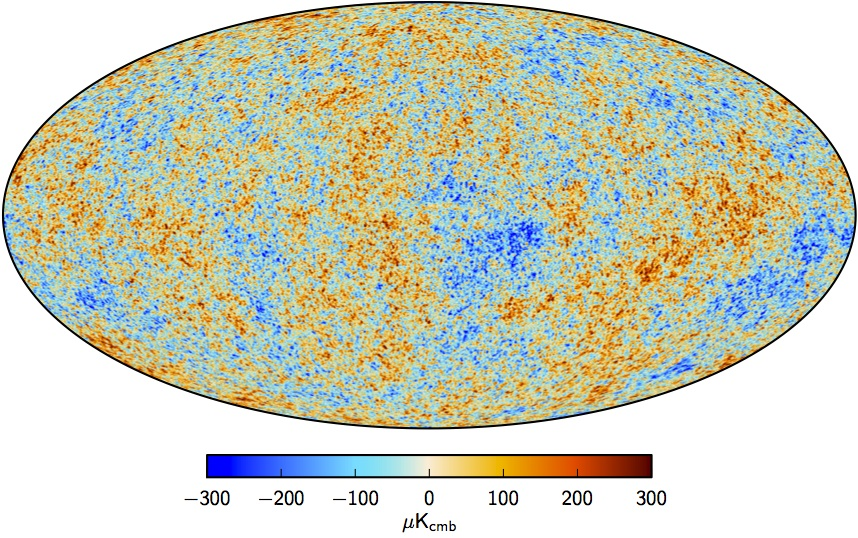
\includegraphics[width=0.47\textwidth]{figs/CMB_PlanckMap.jpg} 
\includegraphics[width=0.47\textwidth, height=165pt]{figs/LSS_SDSS_release14.jpg} \\[5mm]
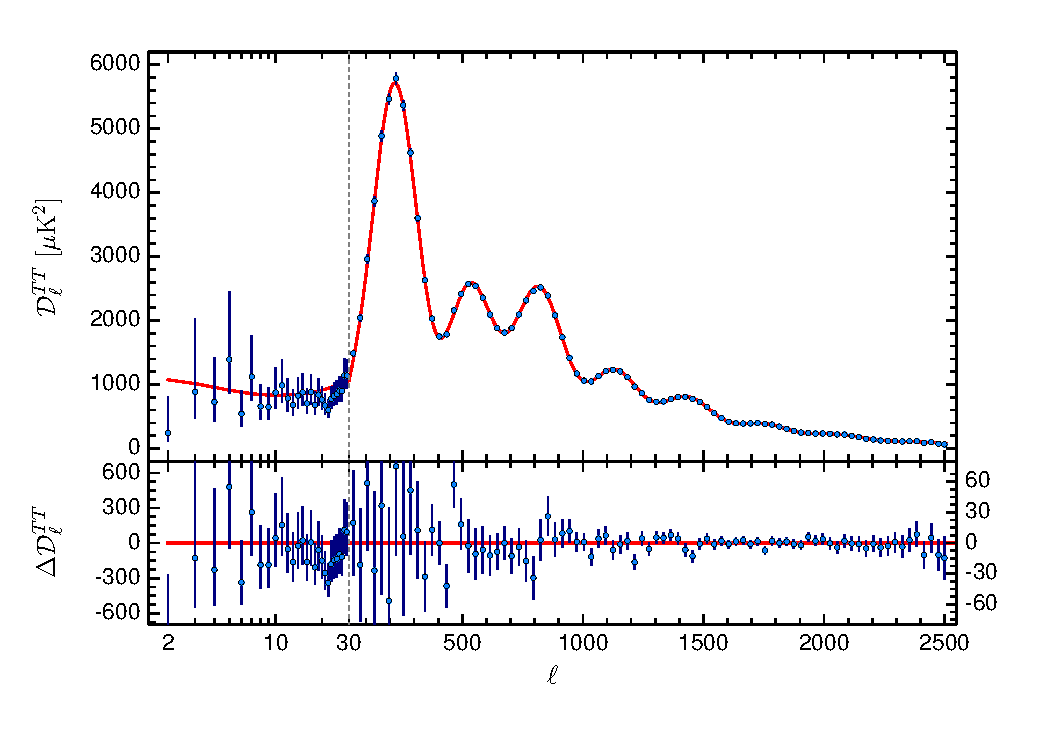
\includegraphics[width=0.47\textwidth]{figs/CMB_Planck2014_TT.pdf} 
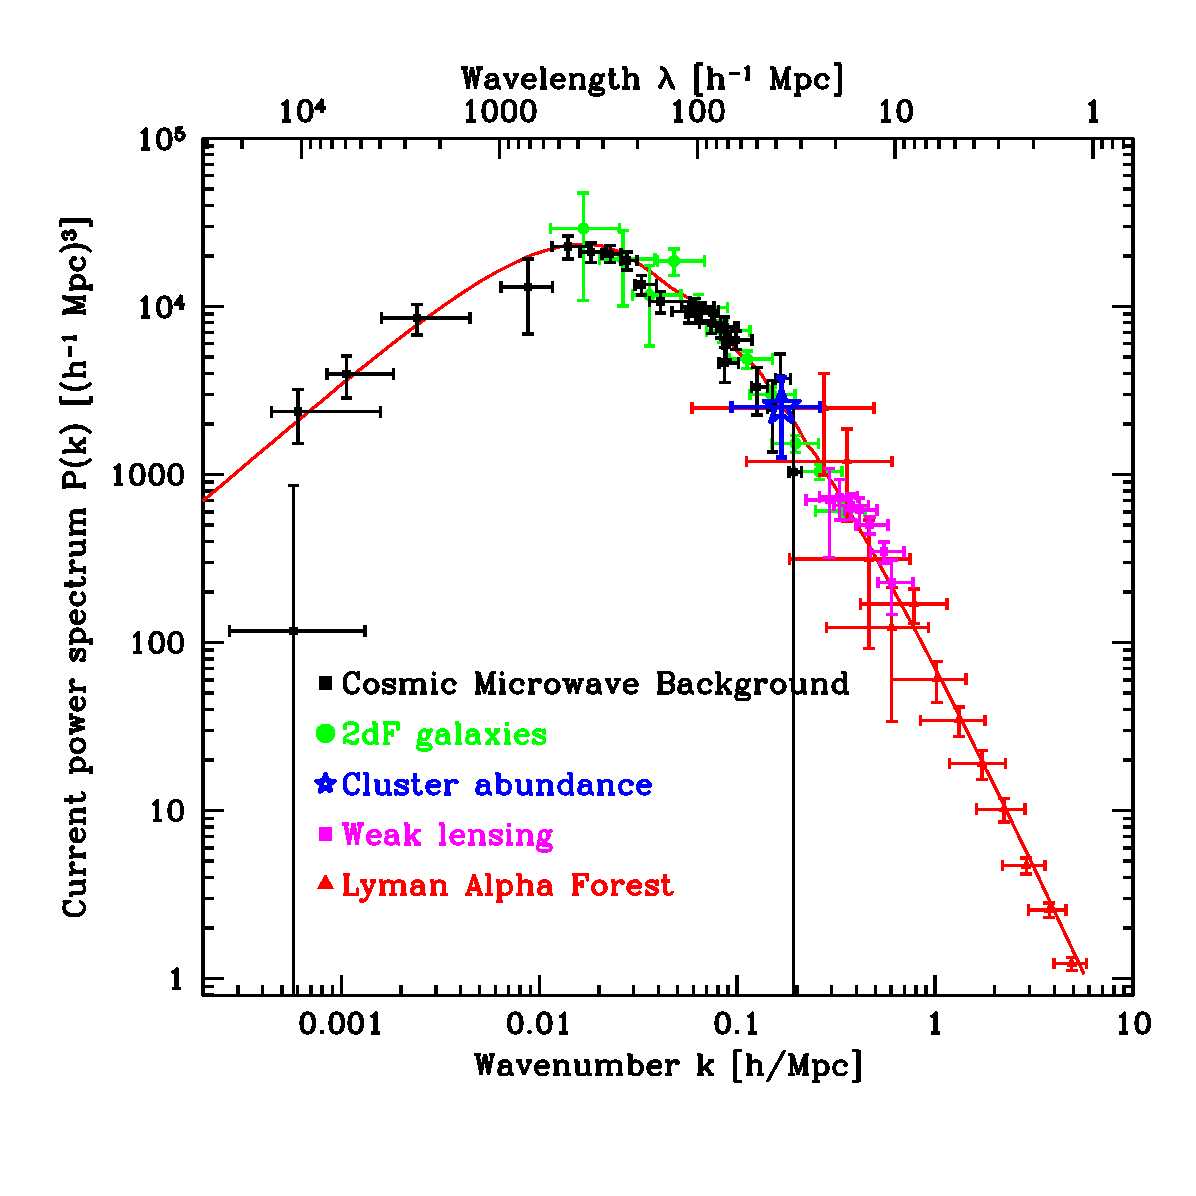
\includegraphics[width=0.47\textwidth, height=170pt]{figs/LSS_powerspectrum.pdf} \\[5mm]
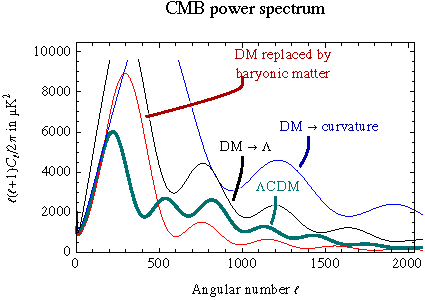
\includegraphics[width=0.47\textwidth, height=170pt]{figs/CMBnoDMAS} \qquad
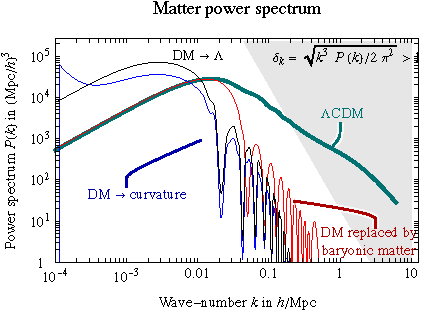
\includegraphics[width=0.47\textwidth]{figs/LSSpowerDMAS} \\
\end{center}
\caption[CMB and LSS]{\em\label{fig:CMBLSS} The  power spectrum of the {\bfseries CMB acoustic peaks} (middle row, left) is extracted from the map of {\bfseries temperature anisotropies} (top left). The {\bfseries matter power spectrum} (middle row, right) is extracted from extensive {\bfseries galaxy surveys} (top right) as well as from other mapping probes. The same quantities in absence of DM are illustrated in the bottom row. 
Figures: from~\cite{Planckresults,LSSCMB}, $\copyright$ESO, $\copyright$APS, reproduced with permission; courtesy of M.~Blanton and SDSS; created with the \href{https://lambda.gsfc.nasa.gov/toolbox/camb_online.html}{{\sc Camb} web interface}.
}
\end{figure}



\subsection{Large scale structure formation}\index{Cold}\index{DM properties!cold}
\label{sec:linear:inhom}\index{Large scale structure}
Today, the Universe is very inhomogeneous on scales smaller than its present horizon.
Take for instance the results of galaxy surveys such as the one shown in fig.~\ref{fig:CMBLSS} (top right), which corresponds to a 3-dimensional map of a good fraction of all galaxies in the observable Universe.
Already by eye one can resolve a variety of structures: lumps, filaments, walls, voids, which appear at  different scales. 
Other astronomical observations, such as the Lyman-$\alpha$ forest, weak lensing measurements, cluster counts, etc, concur in establishing the picture of a 
clumpy Universe. 
Simulations and observations suggest that
voids are regions with density $\sim 10\times$ smaller than the average: they fill $\sim 77\%$ of the volume, while containing only $\sim 15\%$ of the total mass~\cite{1401.7866}.
Walls occupy about $18\%$ of the volume, while containing about a quarter of the mass.
Filaments provide the dominant contribution to gravitational forces: they occupy about $6\%$ of the volume, and contain about half of the mass.
Lumps occupy a small sub-percent fraction of the volume, and contain $\sim 11\%$ of the mass.




Quantitatively, from all these measurements one can extract the {\em matter power spectrum} $P(k)$ plotted in fig.~\ref{fig:CMBLSS} (middle row on the right). It is defined via 
$\langle \delta_k \delta_{k^\prime} \rangle = (2 \pi)^3 \, P(k) \, \delta^3(\vec k- \vec k^\prime)$, where $\delta_k$ is the Fourier transform of the density contrast $\delta(\vec r)$, defined more precisely in eq.\eq{Fourier} below, and $\langle \ \rangle$ denotes an average over $\vec k$ orientations.
The Dirac delta $\delta^3(\vec k- \vec k^\prime)$, not to be confused with the $\delta$ that denotes the perturbations, 
means that modes with different $\vec k \neq \vec k'$ happen to be statistically independent. This property can be understood from inflation, a theory that predicts average statistical properties encoded in $P(k)$.
Since $P(k)$ is the Fourier transform of the density self-correlation function, it conveniently expresses in Fourier space the inhomogeneity in matter distribution in the physical space. A large (small) value of $P(k)$ means that there exist many (few) structures with the characteristic size $\sim 1/k$. The measurements shown in fig.~\ref{fig:CMBLSS} (middle right) therefore show that the Universe has `some power on all scales'. 
To make the clumpiness of the Universe even more apparent, sometimes $P(k)$, which has units of (length)$^3$, is rescaled into the dimension-less  variance $\Delta^2(k) = k^3 P(k)/2 \pi^2$. 
Small values of $\Delta^2$ correspond to small density contrasts, while $\Delta^2 \sim 1$, for instance,  indicates an over-density comparable to the average. A quick manipulation of the $P(k)$ data in fig.~\ref{fig:CMBLSS} (middle right) shows that indeed $\Delta^2$ rises to large values in the large $k$ region. In other words, the data show that the Universe exhibits large inhomogeneities on small scales (large $k$).

In the standard cosmological model
the  primordial inhomogeneities are generated from inflation with  small amplitudes, $\delta \approx 10^{-5}$. 
This is confirmed from the near-perfect smoothness observed in the CMB, which essentially provides 
a photo of the photon content of the Universe, taken when photons last scattered.

This poses a question: how could the tiny primordial inhomogeneities
grow from such small amplitudes to the large contrasts that we observe today?
The answer, as anticipated above, is that the growth of the density perturbations is crucially driven by the presence of DM. In order to quantitatively understand how that happened, we need to sketch their evolution in the early Universe.\footnote{Cosmological perturbation theory and structure formation is a whole research field in itself. Here, we focus only on the aspects that are instrumental to our goal, which is to show the crucial role that DM plays in the growth of such structures. We follow quite closely the treatment found in classic textbooks~\cite{cosmobooks}.}

\medskip

Let us consider a Universe filled with a generic matter fluid, whose exact nature we leave for the moment unidentified.
The main features of the evolution of density perturbations of such a medium can be understood by approximating
the full general-relativistic computation with its Newtonian limit. This is a valid description of non-relativistic matter at length scales smaller than the horizon.
A non-relativistic fluid is fully characterized by its density, $\rho(\vec{r},t)$, by its velocity field, $\vec{v}(\vec{r},t)$ and by the equation of state for the pressure $\wp(\rho)$.
Its gravitational interactions are described by the Newton potential $\Phi$. These quantities are governed by the evolution (`Euler') equations 
\beq 
\label{eq:Euler}
\left\{\begin{array}{ll}
\displaystyle \dder{\rho}{t} +\vec{\nabla}\cdot (\rho\vec{v}) = 0, & \hbox{continuity,}\\[2mm]
\displaystyle \dder{\vec{v}}{t} +(\vec{v}\cdot\vec{\nabla}) \vec{v} =- \frac{\vec{\nabla} \wp}{\rho} - \vec{\nabla}\Phi,
\qquad \qquad & \hbox{Newton law $\vec{a}=\vec{F}/m $,} \\[3mm] 
\displaystyle \nabla^2 \Phi = 4\pi G  \rho, & \hbox{Poisson,}\\
\end{array}\right.\eeq
which form a system of non-linear differential equations. 
For a quasi-homogeneous universe it is possible to gain useful analytic information
by expanding the above quantities as the 1st-order perturbations to a 0th-order homogeneous background
\beq \label{eq:expansioninhom}
\rho = \rho_0(t)+\rho_1(\vec{x},t),\qquad \wp = \wp_0 + \wp_1,\qquad
\vec{v}=\vec{v}_0 + \vec{v}_1 ,\qquad
\Phi = \Phi_0 + \Phi_1.
\eeq 
We first consider the case of a static universe (no expansion). Eq.s~(\ref{eq:Euler}) reduce to a set of coupled equations for the perturbations 
\beq 
\label{eq:Euler1}
\left\{\begin{array}{ll}
\displaystyle \dder{\rho_1}{t} + \rho_0 \vec\nabla \cdot \vec v_1 =0, \\[2mm]
\displaystyle \dder{\vec v_1}{t} + \frac{v_s^2}{\rho_0}  \vec\nabla\rho_1 + \vec\nabla \Phi_1 = 0,  \\[3mm]
\displaystyle \nabla^2 \Phi_1 = 4 \pi G  \, \rho_1,
\end{array}\right. \qquad \hbox{(static Universe)}\eeq
where we defined the quantity $v_s^2 = \partial \wp/\partial\rho = \wp_1/\rho_1$ which is interpreted as the sound speed in the fluid (as we will see in a moment). By acting with $\partial/\partial t$ on the first equation, and performing appropriate substitutions in it using the second and third equations, one arrives at one evolution equation for the density perturbation $\rho_1$, i.e.,~at the {\em Jeans equation},
\beq
\label{eq:fluid0}  
\dder{^2 \rho_1}{t^2} - v_s^2 \nabla^2 \rho_1 = 4\pi G \, \rho_0 \, \rho_1.
\eeq
Ignoring gravity (i.e., setting $G=0$), the solution are density waves (i.e.,~sound) that travel at speed $v_s$. Including gravity, the full equation expresses the competition between a pressure term (on the left-hand side) and a collapse term (on the right). The Jeans length $\lambda_J = \sqrt{v_s^2/(4 \pi G \rho_0)}$ discriminates which term is dominant: perturbations on large scales $\lambda > \lambda_J$  collapse and grow in time, while perturbations on small scales $\lambda < \lambda_J$ are supported by pressure. The growth with time of the collapsed modes is exponential, $\rho_1 \propto e^{\sqrt{4\pi G \rho_0}\, t}$, as one can easily check by solving the differential equation \eqref{eq:fluid0} for $v_s\to0$. 
This is the Jeans instability that, when applied to normal matter, explains how gas clouds collapse to form compact bodies, e.g.,~stars.
The intuitive meaning of the Jeans scale is that a cloud of gas collapses when it is so big that its hydrostatic pressure, 
which prevents the collapse on time-scales $\tau_{\rm pressure} \sim \lambda_J/v_s $,
is too slow to stop the gravitational attraction, which clumps it on a time-scale  $ \tau_{\rm gravity}\sim (G \rho_0)^{-1/2}$.
One can also define the Jeans mass as $M_J = 4\pi \rho_0 \lambda_J^3/3$, i.e.,  as the mass enclosed in a sphere of radius $\lambda_J$. Perturbations with mass $M > M_J$ are `Jeans unstable' and  collapse.

\medskip

We move next to the  case of an expanding universe. 
Solving the 0th-order quantities describing the smooth background gives the Hubble expansion
\beq\label{eq:rho0(t)}
\rho_0(t) = \frac{\rho_0(t_0)}{a^3},\qquad
\vec{v}_0 = H \vec{r},\qquad
\vec{\nabla}\Phi_0 = \frac{4\pi G\rho_0}{3}\vec{r}.
\eeq
So far, $a(t)$, the usual scale factor of the Universe, has been left with an unspecified time dependence.
Solving eq.s~\eqref{eq:Euler} would determine the expansion $a(t)$ of a matter-dominated universe.
In general, extra components (radiation and the cosmological constant) contribute to the expansion,
and $a(t)$ is given by the fully relativistic Friedmann equations, see Appendix \ref{app:Cosmology}.
The first relation in \eqref{eq:rho0(t)} is just the standard dilution of non-relativistic matter when the volume expands by a factor of $a^3$. 
The second relation is the Hubble law for the velocity field of the homogeneous background, with respect to which the perturbations $\vec v_1$ can be seen as peculiar velocities. 
The third is the solution to the Poisson equation, applying the Gauss theorem to a sphere with radius $r$
centered at the origin and ignoring the infinite amount of outside matter;
this logical jump, known as the `Jeans swindle', is justified thanks to the existence of a horizon in the full relativistic treatment.\index{Jeans swindle}

\smallskip

Expanding eq.~(\ref{eq:Euler}) to 1st-order  in the perturbations leads, after
tedious but straightforward derivations, to the linear equations
\beq 
\label{eq:Euler2}
\left\{\begin{array}{l}
\displaystyle \dder{\rho_1}{t} +3H \rho_1 + H (\vec{r}\cdot \vec{\nabla})\rho_1+
\rho_0  \vec{\nabla}\cdot \vec{v}_1 = 0,\\[2mm]
\displaystyle \dder{\vec{v}_1}{t} +H \vec{v}_1 + H(\vec{r}\cdot \vec{\nabla})\vec{v}_1 + \frac{v_s^2}{\rho_0} \vec{\nabla}\rho_1
+\vec{\nabla}\Phi_1=0,\\[1mm]
\displaystyle \nabla^2 \Phi_1 = 4\pi G \rho_1,
\end{array}\right. \qquad \hbox{(expanding Universe).}
\eeq
The extra terms in eq.~(\ref{eq:Euler2}), as compared to eq.~(\ref{eq:Euler1}), are identified by the appearance of $H$.
Next, we define the relative density (or density contrast) $\delta(\vec r)$ and expand it in co-moving Fourier modes:
\beq 
\label{eq:Fourier}
\delta(\vec{r}) \equiv \frac{\rho_1(\vec{r})}{\rho_0} =\int  \frac{d^3k}{(2\pi)^3}\,\delta_k(t) \exp\left[{- i\vec{k}\cdot\vec{x}}\right],\qquad {\rm where} \quad
 \vec{x} \equiv\displaystyle \frac{\vec{r}}{a(t)}.
\eeq
The rescaling of the space vector by a factor $a(t)$ means that the wavenumber $1/k$ follows the average evolution of the universe. This is  convenient because, in this way, equations
for modes $\delta_k$ with different $k$ turn out to be decoupled.  Similarly, we define $\vec v_k$ and $\Phi_k$, the Fourier transforms of the velocity perturbation $\vec v_1$ and of the gravitation potential $\Phi_1$. In Fourier space eq.~(\ref{eq:Euler2}) becomes
\beq 
\label{eq:EulerF}
\left\{\begin{array}{l}
\displaystyle \dder{\delta_k}{t} -\frac{i\vec k}{a}\cdot \vec v_k  = 0,\\[3mm]
\displaystyle \dder{(a \, \vec v_k)}{ t} -i \vec k v_s^2 \delta_k - i \vec k \Phi_k =0,  \\[2mm]
\displaystyle \Phi_k = -\frac{4 \pi G \rho_0}{k^2} a^2 \, \delta_k.
\end{array}\right. 
\eeq
The second equation in \eqref{eq:EulerF} can be simplified further. One can decompose the velocity perturbation as $\vec v_1 = \vec v_{1\perp} + \vec v_{1\parallel}$, where $\vec \nabla \cdot \vec v_{1\perp} =0$ (divergence-free or solenoidal component) and $\vec \nabla \times \vec v_{1\parallel} =0$ (curl-free or irrotational component). In Fourier space $\vec k \cdot \vec v_{k\perp} =0$, $\vec k \times \vec v_{k\parallel} =0$. The second equation in (\ref{eq:EulerF}) for $\vec v_{k\perp}$ just amounts to $\partial(a \, \vec v_{k \perp})/\partial t =0$, giving $\vec v_{k \perp} \propto 1/a$. The solenoidal component $\vec v_{k\perp}$ therefore  dies away with the expansion of the Universe, and only the irrotational component, $\vec v_{k\parallel}$, survives. Since $\vec v_{k\parallel}$ is parallel to $\vec k$, we can substitute everywhere in eq.~(\ref{eq:EulerF}) $\vec{v}_{k} \to v_k \hat{\mb{k}}$ (where $\hat{\mb{k}}$ is the unit vector along $\vec k$) 
and $\vec k \to |\vec k| \equiv k$. At this point we can combine the three equations \eqref{eq:EulerF} into one second order equation. By taking $v_k$ from the first equation, plugging it into the second and using $\Phi_k$ from the third, we arrive at 
\beq
\label{eq:deltaDM}
\frac{\partial^2\delta_k}{\partial t^2}  + 2H \frac{\partial\delta_k}{\partial t} + \left(\frac{v_s^2 k^2}{a^2} - 4\pi G \rho_0\right) \delta_k=0. 
\eeq
This is the Jeans equation for density perturbations, analogous to eq.~(\ref{eq:fluid0}) but in the Fourier space and for a  Universe that is expanding with Hubble parameter $H$.
Similarly to the static case, 
the pressure term (proportional to $v_s^2$) wins over the collapse term (proportional to $G \rho_0$) 
for small length scale modes, i.e., for  $k> k_J \equiv a \sqrt{4 \pi G \, \rho_0/v_s^2}$.
The critical Jeans wavenumber $k_J$ now depends on $a$, indicating that different scales start clustering at different times.
Furthermore, the expansion of the Universe 
has a friction-like effect (the extra term in \eqref{eq:deltaDM} proportional to $H$)  and thereby slows the clustering of matter.


\medskip


It is now time to specify which kind of matter fluid we are dealing with, and in which epoch of the Universe's evolution it is relevant. 


\paragraph{Non-clustering of baryonic matter.} Before considering Dark Matter, let us first focus on the case of baryonic matter coupled to photons.
This means that the protons (as well as nuclei) and the electrons, which in cosmology are collectively called the `baryonic matter', 
are {\em tightly coupled} by electromagnetism to the photons. They form a matter fluid with the relativistic sound speed $v_s \approx  c/\sqrt{3}$, where $c=1$ is the speed of light.
With this extra input from relativistic physics, we can then proceed with the non-relativistic Jeans equation for density perturbations, eq.~(\ref{eq:deltaDM}).
The large speed of sound, $v_s \sim\mathcal{O}(1)$,  means that the large pressure provided by photons dominates over the gravitational term in eq.~(\ref{eq:deltaDM}).
One thus expects that such a fluid does not cluster.
This is confirmed by the explicit solutions of eq.\eq{deltaDM}.
In a matter-dominated universe, i.e., in the case most favourable for clustering since radiation does not cluster, one has 
$\rho_0 = 3H^2/8\pi G$, 
$a(t)=(\frac32 tH_0)^{2/3}$ and 
$H = \dot a/a = \sfrac{2}{ 3t}$, see Appendix \ref{app:Cosmology}. Eq.~(\ref{eq:deltaDM}) then becomes
\beq\label{eq:acoustic}
\frac{\partial^2\delta_k}{\partial t^2} + \frac{4}{3t} \frac{\partial \delta_k}{\partial t} + \frac{v_s^2 k^2}{ \left( \frac32 H_0 \right)^{4/3}\, t^{4/3}}  \delta_k=0,  \qquad\hbox{giving}\qquad 
\delta_k = \frac{c_1 \cos(c_0  \, k  t^{1/3}) +c_2 \sin(c_0 \, k  t^{1/3})}{k \, t^{1/3}}.
\eeq
For simplicity we do not specify the coefficients $c_0$, $c_1$ and $c_2$, which depend on $v_s$ and $H_0$.
The main result is that this solution is {\em oscillating} 
(pressure waves, observed as peaks in the CMB power spectrum)
and {\em damped} in time. 
The baryonic tightly-coupled fluid does not cluster on scales $k> k_J (a) \sim aH/v_s$, with the latter equal to the horizon,
given that $v_s\sim \mathcal{O}(1)$.
In other words, normal matter without Dark Matter only clusters at late times, after it decouples from photons.


\paragraph{Clustering of Dark Matter.}
What makes Cold Dark Matter different is that it does not interact with photons and is collectively described by a
simple fluid with non-relativistic sound speed, $v_s = 0$. This makes a huge difference in cosmology.
Keeping only the gravity term in eq.~(\ref{eq:deltaDM}) and considering again the matter-dominated phase of the Universe, one obtains
\beq\label{eq:deltaDM(t)}
\frac{\partial^2 \delta_k}{\partial t^2} + \frac{4}{3t}\frac{\partial \delta_k }{\partial t}- \frac{2}{3t^2} \delta_k=0,\qquad\hbox{giving}\qquad \delta_k = c_{\rm grow}~ t^{2/3}+
c_{\rm decay}~ t^{-1}.
\eeq
This solution contains a decaying mode that dies off, and, most importantly, 
contains a mode that grows with a specific positive power of time.
This is how the Universe evolved from a primordial quasi-homogeneous state with $\delta_k \sim 10^{-5}$ to the present clumpy state.
Incidentally, note that the exponential growth found in the static case has become a power-law growth in
the expanding Universe: expansion acts like a brake that slows down the clustering.

\medskip

For completeness, we can also consider the DM fluid in the Radiation-Dominated (RD) epoch, described by $H=\sfrac{1}{2t}$. In this case, one can show that eq.~(\ref{eq:deltaDM}) loses both the $v_s^2 k^2 \delta_k/a^2$ term (because $v_s = 0$ for the DM fluid) and the $4\pi G \rho_0 \delta_k$ term (because the relevant $\delta_k$ would be the one of radiation, which however does not cluster and therefore does not source perturbations in the gravitational potential).  Eq.~(\ref{eq:deltaDM}) therefore reduces to
\beq 
\frac{d^2\delta_k}{dt^2} + \frac{1}{t}\frac{d\delta_k}{dt} =0,\qquad\hbox{giving}\qquad \delta_k \propto \ln t +\hbox{const}.
\eeq
Hence, DM perturbations grow only logarithmically during radiation domination. Similar computations show that DM does not  cluster efficiently when the Universe is dominated by the vacuum energy, or by curvature.


\medskip

In summary, the standard history of structure formation is as follows. The Universe became matter-dominated when the scale factors was $a_{\rm eq} \sim 1/3400$.  
At that point, primordial DM inhomogeneities $\delta_k \sim 10^{-5}$ 
began to grow as $t^{2/3} \propto a$ on length scales $1/k$ which are 3400 times smaller than the present horizon.
Larger length scales started clustering later, as soon as they became smaller than the expanding horizon.
During matter domination a mode $k$ re-entered the horizon when the scale factor was $a_k \approx H_0^2/k^2$.
Up to ${\mathcal O}(1)$ factors, this result follows from imposing $k/a_k \approx H(a_k) = H_0 \sqrt{\Omega_m/a_k^3}$.
At present time we then have
\beq \delta_k  \approx 10^{-5} (a_0/a_k) \approx 10^{-5} (k/H_0)^2,\label{eq:deltaktoday}
\eeq
which is larger than unity on scales $H_0/k \lesssim  10^{-5/2}$, about 3 orders of magnitude smaller than the current horizon.


Normal matter, in contrast, could not cluster because it was tightly coupled by electromagnetism to photons and was forming pressure waves.
Later in the evolution of the Universe, at $a_{\rm recomb}\sim 1/1100$, 
the temperature became low enough, and the photon bath diluted enough, that electrons and positrons could bind to form neutral hydrogen. At that point normal matter decoupled from radiation and began falling into the gravitational potential wells that DM had already started to form. 
In this sense, DM is a key ingredient in the construction of the `cosmic scaffolding' observed in the Universe.

The observed matter power spectrum $P(k)$, or, equivalently, the variance $\Delta^2(k)$, corroborate this history. 
If the Universe contained baryonic matter only, perturbations would have had a much smaller power and would have exhibited much more pronounced oscillations (bottom right panel of fig.~\ref{fig:CMBLSS}), in clear disagreement with the observations. A Universe containing the `right mix' of baryons and DM, i.e.~in the proportions given in eq.~(\ref{eq:OmegaDMh2}), agrees with  data. The power spectrum changes slope at 
$k \gtrsim 3400 \, \Omega_{\rm rad} H_{0} \sim 10^{-2}/{\rm Mpc}$ corresponding to scales entering the horizon at 
matter/radiation equality 
and therefore undergoing the growth during matter domination. 
On top of the smooth function, the small wiggles around $k \approx 0.1 \ h$ Mpc$^{-1}$, called {\em `baryonic acoustic oscillations'} (BAO), are the imprints of pressure waves due to the subdominant population of baryons. \index{Baryonic acoustic oscillations}



\medskip

As an aside, an important lesson of the above formalism is that Dark Matter made of objects with sizeable speed $v$
would not be described by $v_s=0$ --- rather, it would diffuse, suppressing the small-scale inhomogeneities.
Observational data therefore constrain the DM temperature,  or equivalently, the average kinetic energy of DM, to be much smaller  than the DM mass.
For thermalized particles, this means $M \circa{>}{\rm keV}$, as discussed  in section \ref{sec:WarmDM}.


\begin{figure}[!t]
\begin{center}
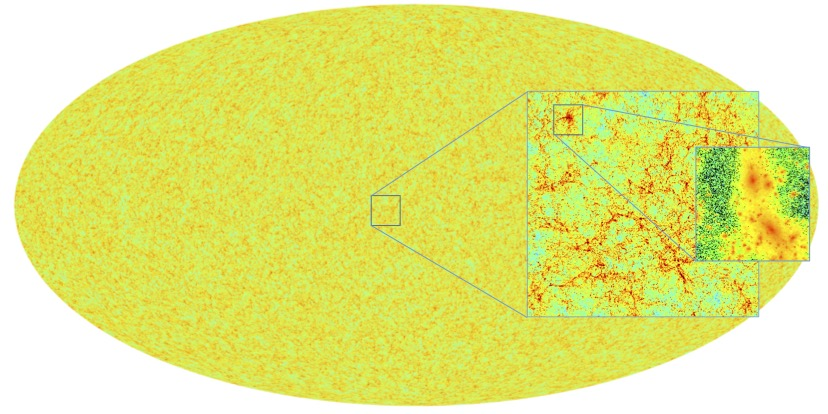
\includegraphics[width=0.7\textwidth]{figs/NbodyPotter2016} 
\end{center}
\caption[$N$-body simulation]{\em\label{fig:Nbody}
Results from a full-sky ${\mb N}${\bf-body DM simulation} (from~Potter et al.\ in~\cite{Nbody}).}
\end{figure}



\subsection{Non-linear growth of inhomogeneities: numerical simulations}\label{Nbody}\index{Numerical simulations}
The previous subsection discussed analytically 
how primordial density perturbations $\delta_k $ grow due to gravitational attraction, 
in the perturbative limit $\delta_k\ll 1$. 
Over-densities eventually reach $\delta_k \sim 1$ so that the perturbative computation no longer applies. 
At this point gravitationally bound systems start to form: galactic subhalos, galaxies, clusters of galaxies, etc.
{\em Smaller structures form first}, 
as inhomogeneities $\delta_k (t)$ are larger at smaller scales $1/k$ (see above). Larger structures form later, from accretion of diffuse DM and from merging of pre-existing smaller structures (this process is referred to as {\em hierarchical structure formation}).\footnote{The density of forming structures is roughly given by the cosmological density at the formation time, therefore smaller structures have higher density, in agreement with fig.\fig{catalogue}.} 
\index{Boltzmann equation}
The dynamics of the growth is still described by the gravitational collision-less Boltzmann equations, written in the Eulerian form in eq.\eq{Euler}, but now the non-linear effects become relevant. 
The study of the evolution of inhomogeneities beyond $\delta_k\sim1$ is therefore done via computer simulations~\cite{Nbody}. 
These are a remarkable feat as they are able to cover huge ranges: $\sim$$10^{13}$ years in time (from initial conditions at $z \approx 100$, $t\approx 10$ Myr to $z\approx0$ today), $\sim$7 orders of magnitude in space (some recent simulations deal with volumes of $\mathcal{O}(10 \,{\rm Gpc})^3$ with $\sim$kpc resolution), $\sim$11 orders of magnitude in density contrast (from $\delta_k \approx 10^{-5}$ at recombination to $\delta_k \approx 10^{6}$, the typical density contrast in collapsed large scale structures today) and up to $\sim$30 orders of magnitude in mass (the recent simulations by \arxivref{1911.09720}{Wang et al.~(2020)}~\cite{Nbody} are able to resolve at the same time Earth-mass halos, $\sim10^{-6}M_\odot$, and cluster-mass halos, $\sim10^{14}M_\odot$, and they can trace $10^{-11}M_\odot$ elements within a total simulated mass of $10^{19}M_\odot$, thanks to multi-zoom techniques).  
 
What is done in practice is to simulate the gravitational motion of a large number $N$ of massive points (hence the name {\bf $\mb{N}$-body simulations}) moving in the expanding background of the Universe, starting from typical realizations of the primordial inhomogeneities.
Present computers can solve Newtonian equations of motion for $N\sim 10^{12}$ massive points.\footnote{Approximations based on multipoles and dedicated techniques 
allow the reduction of their $N^2$ gravitational forces computation to an ${\cal O}(N)$ numerical complexity.
Furthermore, the gravitational forces are softened on small scales to avoid
unphysical scatterings among nearby particles due to numerical issues.
The simulations are performed assuming periodic boundary conditions.}
While elementary DM particles are much more numerous, 
thanks to the universal nature of gravity this is enough to simulate properly the physics on scales bigger than the size of a single element,
where the mass of each element is ${\cal M}/N$, with ${\cal M}$ the total mass in the computed volume.

\index{Numerical simulations!cosmic web}
At the qualitative level, such simulations produce images and movies that show how DM clusters into filaments, walls and pancakes that merge in halos separated by voids, producing what is often referred to as the {\em cosmic web}, see fig.\fig{Nbody}. 
For instance, they show how objects with total mass $\approx 10^{12}M_\odot$, such as the Milky Way, mostly form at redshift $z\approx 1$, while presently about $20\%$ of the DM remains diffuse.
At the quantitative level, simulations allow to predict statistical properties of the formed structures:
the distribution in mass (the halo mass function), the typical shape (spherical or ellipsoidal), the typical density profiles $\rho(r)$, the DM velocity distribution and its variance $\sigma^2(r)$.
We will return to these quantities when discussing detailed results about the DM distribution in section~\ref{sec:resNbody} and~\ref{sec:DMdistribution},
and possible anomalies in section~\ref{CDMproblems}. 
The claim here is more general: the Dark Matter hypothesis leads to an
overall agreement between the qualitative and quantitative results of these simulations and the observed properties of the large scale structure in the current Universe.
As hinted to several times already, DM is the scaffolding that shapes and supports the distribution of the visible matter in the Universe. Numerical simulations are instrumental in testing its presence because they provide the essential link between theoretical models for the origin and evolution of cosmological structure and the actual astronomical observations.


\medskip

The discussion so far has concerned DM-only numerical simulations, performed since the 1980's. Ordinary matter (a.k.a.~`baryons') is less abundant than DM, but its effects are very important and should be included, which is what recent simulations (called {\bf baryonic} or {\bf hydrodynamical simulations}) started to do, trying to achieve precision~\cite{Sims_with_baryons}.\index{Numerical simulations!baryons} 
Discussing in detail how these simulations model baryons and their interactions goes beyond the focus of our review. In general terms, these simulations need to take into account a large number of different physical processes, on different time-scales and for very large ranges of velocities, densities, temperatures, viscosities, etc. 
The ingredients include: gas hydrodynamics,
gas cooling, radiation, magnetic fields (since these significantly contribute to pressure; their amplification, included in the computer codes,
presumably makes their more complicated seeds irrelevant),
star formation and star death, as well as the dynamics of stellar ejecta (including supernov\ae{}:
the resulting cosmic rays contribute to pressure in the interstellar medium and significantly change the gravitational potential by moving matter from a localized center to a wide surrounding region within a short timescale),
 super-massive black holes (present in massive galaxies; their seeds are not known, they presumably grow acquiring gas, with possible mergers), etc.
 Dust, thermal conduction and viscosity are believed to be less important.

As a result, the computer codes recently started to produce realistic galaxies.
While the details vary (for example, the formation of spirals critically depends on how stellar feedback regulates star formation), different codes presently seem to agree on a number of predictions.
The overall conclusion seems to be that the $\Lambda$CDM model including baryons can account for galaxy formation and
that the basic physics that shapes galaxies has been identified.
Such codes do contain, however, freely adjustable parameters, including those that control the numerical approximations, such as the spatial resolution and the modelling of the so-called `sub-grid physics'. As such, there is the usual danger of possibly (over)fitting data to the incomplete or even incorrect models, where adjusting the phenomenological parameters may mimic the effects of something else. 

Numerical simulations also include Dark Energy (DE), at least in the form of an accelerated expansion of the underlying Universe, hence entering in the background Hubble parameter at late times~\cite{Sims_DE}. Alternative models of DE are also simulated. The effect on structure formation can be sizable, but it is not always easy to disentangle it from other degenerate effects. 

\medskip

Finally, we mention that numerical simulations can be used to study the nature of Dark Matter, i.e., to explore the deviations from the assumption of the vanilla cold, collisionless DM. For instance, numerical simulations of warm DM, self-interacting DM and fuzzy DM, with or without baryons, have been performed~\cite{Sims_alt_DM}. 
We will come back to some of the constraints imposed by these simulations in sections \ref{sec:DMparticle} and \ref{ultralight}.
In this context, a powerful tool is the {\sc Ethos} framework \cite{ETHOS}. {\sc Ethos} (the Effective THeory Of Structure formation) is a scheme in which the different microphysical DM interactions are translated into general effective parameters that modify the perturbation equations discussed in section \ref{sec:linear:inhom}. Hence in principle performing one {\sc Ethos} numerical simulation, with a chosen set of effective parameters, allows to constrain all the microphysical models captured by such a set.



\subsection{CMB acoustic peaks}\label{sec:CMB}\index{CMB}
In this section we discuss how the cosmic microwave background (CMB) carries the imprint of the presence of DM. 
The chief observable is the CMB power spectrum (middle left panel in fig.~\ref{fig:CMBLSS}): it is 
obtained by performing a spherical Fourier transform of the photon temperature field (the anisotropies in the top left panel of the same figure), 
and then computing the variance by averaging over the $2\ell+1$ orientations for each value of the angular momentum, $\ell$.
This variance is measured and is compared to the predictions of inflationary big-bang cosmology:
such comparison allows to infer information on the contents of the Universe, including, crucially, on the presence of DM.

\smallskip


A bit more precisely, the CMB peaks are due to acoustic oscillations of the baryon/photon fluid, eq.\eq{acoustic}. 
The positions of such acoustic peaks depend on the DM density (less DM means later radiation-matter equality), and their amplitude depends on the relative amount of DM with respect to normal matter (only the latter undergoes acoustic oscillations).
Global fits find that these and other cosmological observables can be well reproduced by the Standard Model of cosmology including DM 
($\Lambda$CDM with adiabatic Gaussian primordial inflationary perturbations), and allow to determine the values of its cosmological parameters. 
This gives the most accurate determination of the DM density $\Omega_{\rm DM}$ currently available.

Below, we expand on this discussion and show semi-quantitatively how DM affects the shape of the CMB power spectrum.  
We over-simplify the physics and focus only on the main DM-related features; a complete discussion can be found in~\cite{CMB:reviews}.

\medskip

The CMB power spectrum has the same intuitive meaning as the matter power spectrum $P(k)$, section~\ref{sec:linear:inhom}, but now for photon anisotropies. Roughly, $C_\ell$ is the amount of anisotropy at angular size $\theta \sim \pi/\ell$.
An angular scale $\theta$ roughly corresponds to wave-number $k \sim \ell H_0$, where $H_0$ is the present Hubble constant.
The CMB power spectrum declines as $\ell$ increases, due to `Silk damping', i.e.,~the smoothing of small scale structures due to photon diffusion~\cite{SilkDamping}. However, the 2$^{\rm nd}$ and the 3$^{\rm rd}$ CMB peaks have roughly equal size. This suggests that, were one able to remove the Silk damping, the 3$^{\rm rd}$ peak would have been particularly prominent and higher than the 2$^{\rm nd}$ peak. This is the footprint of DM, as we proceed to illustrate. 

\medskip

Inhomogeneities in the photon fluid at a particular position $\vec r$ in the Universe and at time $t$ are fully described by a function denoted $\Theta(\vec r, t, \hat{\mb{p}})\equiv \delta T/T$, or equivalently by its Fourier transform $\Theta(\vec k, t, \hat{\mb{p}})$. Here $T$ is the photon temperature and $\hat{\mb{p}}$ is the photon direction. 
This function obeys the following Boltzmann evolution equation~\cite{cosmobooks}\footnote{\label{footnote:CMB:potentials}  
Deriving this equation from first principles is well beyond our intended scope. The reader is invited to consult the classic books in~\cite{cosmobooks}. Note that here we also neglect the photon polarization. It is as well worth mentioning that our notation differs from the one used by Dodelson~\cite{cosmobooks}. First, we denote the Newton potential with $\Phi$, consistent with section~\ref{sec:linear:inhom} (and with Kolb \& Turner and Weinberg~\cite{cosmobooks}), and the curvature perturbations with $\Psi$, hence $\Phi \leftrightarrow \Psi$ when comparing our formalism with Dodelson's. Second, $k \to -k$ because of a sign difference in the convention of Fourier transforms (see eq.~(\ref{eq:Fourier})). Third, Dodelson denotes with $\dot{} \equiv d/d\eta$ the derivative with respect to conformal time, while in our notation (again consistently with Kolb \& Turner and Weinberg~\cite{cosmobooks}) $\dot{} \equiv d/dt$ and $^\prime \equiv d/d\eta$, hence $X^\prime = a  \,\dot{X}$ in our notation.
Finally, in this section we use the $(-+++)$ metric, see eq.\eq{metricPhiPsi}, which is convenient in cosmology and thus eases comparison with the literature.
In the later sections we will use the $(+---)$ metric, convenient for particle physics.}
\beq
\label{eq:BoltzmannEqphotonsmain}
\dot \Theta -i \frac{k}{a} \mu \Theta + \dot  \Psi -i\frac{k}{a} \mu \Phi = - \dot \tau\left[ \Theta_0 -\Theta + \mu v_{{\rm b}k} \right],
\eeq
where $\mu=\hat{\mb{k}}\cdot \hat{\mb{p}}$ is the angular variable, $\Phi$ is the Newton potential and $\Psi$ is the curvature perturbation, 
appearing in the metric
\beq \label{eq:metricPhiPsi}
ds^2 = -(1+2 \Phi) dt^2 + a^2 d\mb{x}^2 (1+2\Psi).\eeq
Finally, $v_{{\rm b}k}$ is the velocity perturbation of $b$aryonic matter, further discussed below. 
The left terms describe how photons move in the gravitational background; the right terms describe
how photons electromagnetically interact with baryonic matter: the optical depth $\tau$ is defined later.
It is convenient to expand $\Theta$ in multipoles in terms of the Legendre polynomials $\mathcal{P}_\ell$ in the variable $\mu$. The multipoles are denoted as $\Theta_\ell$ and defined as 
\beq
\label{eq:multipolesphotons}
\Theta_\ell =i^\ell  \int_{-1}^{1} d\mu \frac12\mathcal{P}_\ell(\mu) \Theta(\mu).
\eeq
The first two moments, the monopole $\Theta_0(\vec k, t)$ and the dipole $\Theta_1(\vec k, t)$, describe respectively the overall density inhomogeneity and the velocity of the photon fluid, while the higher moments have a less intuitive meaning.

In other words, the evolution of the perturbations in the photon fluid can be described either via the whole function $\Theta(\vec k, t, \hat{\mb{p}})$ or via an infinite array of multipoles  $\Theta_\ell(\vec k, t)$ obeying an infinite array of (coupled) equations derived from eq.~(\ref{eq:BoltzmannEqphotonsmain}).
We now discuss which equations these functions obey during the various phases of the Universe. In particular, a key moment is the epoch of recombination, $a_{\rm recomb}\approx 1100$, i.e.~the point in time when the electrons, protons and neutrons in the plasma formed bound hydrogen and helium atoms.
The photons experience a very different evolution before and after this moment. Before recombination the photons constantly scatter on the charged particles, forming a single {\em tightly coupled baryon-photon} fluid which is non-relativistic. 
For such a fluid, the Boltzmann equations can be truncated, i.e.~only the first two moments introduced above, $\Theta_{0}(\vec k, t)$ and $\Theta_{1}(\vec k, t)$, are needed, while higher moments can be neglected. 
After recombination, photons free-stream from the {\em surface of last scattering}. 
They are a relativistic fluid and the higher multipoles have to be reintroduced, as we will do later.


\subsubsection*{Tightly coupled regime}
In the tightly coupled regime, the evolution of the perturbations in the photon fluid is governed by the two coupled Boltzmann equations for $\Theta_0$ and $\Theta_1$, which are in turn coupled to the evolution equations for matter. The system reads\footnote{The passages to obtain the equations for $\Theta_0$ and $\Theta_1$ from the eq.~(\ref{eq:BoltzmannEqphotonsmain}) for $\Theta$ consist in multiplying eq.~(\ref{eq:BoltzmannEqphotonsmain}) by $\mathcal{P}_\ell$ and doing the integrals over $\mu$ as per the definition of the multipoles in eq.~(\ref{eq:multipolesphotons}), using when needed the recursive relation among the Legendre polynomials: $(\ell+1) \mathcal{P}_{\ell+1}(\mu) = (2 \ell+1)\mu \mathcal{P}_\ell(\mu) - \ell \mathcal{P}_{\ell-1}(\mu)$ \cite{cosmobooks}.}
\beq
\label{eq:BoltzmannEqsDM}
 \left\{\begin{array}{l}
\displaystyle \dot \delta_k -i \frac{k}{a} v_k +3 \dot \Psi_k = 0,\\[3mm]
\displaystyle a  \dot v_k + \dot a v_k - i k \Phi_k =0,
\end{array}\right. \hspace{22ex} {\rm DM~~~~~}
\eeq
\beq
\label{eq:BoltzmannEqsB}
 \left\{\begin{array}{l}
\displaystyle \dot \delta_{{\rm b}k} -i \frac{ k}{a} v_{{\rm b}k} +3 \dot \Psi_k = 0,\\[3mm]
\displaystyle a  \dot v_{{\rm b}k} + \dot a v_{{\rm b}k} - i k \Phi_k = a  \frac{\dot \tau}{R}\big[ 3 i \Theta_1+v_{{\rm b}k} \big] ,
\end{array}\right.\qquad{\rm baryons}
\eeq
\beq
\label{eq:BoltzmannEqsPh}
\left\{\begin{array}{l}
\displaystyle \dot \Theta_0 -\frac{k}{a}\Theta_1 + \dot \Psi_k = 0,\\[3mm]
\displaystyle \dot \Theta_1 +\frac{k}{3a} \Theta_0 + \frac{k}{3a}\Phi_k = \dot \tau \left[ \Theta_1 - \frac{i v_{{\rm b}k}}{3} \right], 
\end{array}\right.\qquad{\rm photons} 
\eeq
with extra equations for neutrinos and for gravity (described by two scalar potentials $\Phi$ and $\Psi$ in the relativistic treatment) which we do not write down for simplicity.
Here $R = 3\rho_{\rm b}/4\rho_\gamma$ and $\tau = \int d\eta \, n_e \sigma_{\rm T} a$ is the optical depth, 
expressed in terms of the number density of electrons $n_e$, of the Thomson cross section $\sigma_{\rm T}$
and of proper time $\eta$ (see appendix~\ref{app:Cosmology}).  
A few comments are in order. The equations for matter (baryons or DM) should look familiar: they correspond to those derived in eq.~(\ref{eq:EulerF}), with a couple of differences: we are here considering the full relativistic treatment, 
so that the perturbation to curvature $\Psi_k$ now appears (the gravitational potential $\Phi$ is still present); 
we made the coupling between baryons and photons explicit with the Thomson scattering term (right side of eq.~(\ref{eq:BoltzmannEqsB})). As expected, the only difference between DM and baryons is the coupling to photons. 
The right side of the second equation in (\ref{eq:BoltzmannEqsPh}) is again the Thomson scattering term that couples photons to baryons. 

\medskip

The above equations show that photons are coupled to matter in two ways: via electromagnetism, as expressed by Thomson scattering, and via gravity, as expressed by the gravitational potentials $\Phi$ and $\Psi$ that appear in the equations for all fluids. 
The coupling to gravity accounts for the physical effect that photons get red-shifted (blue-shifted) when climbing out of (fall in) the gravitational potential wells created by matter. 
The crucial point is thus that the CMB photons are separately sensitive to {\em matter that gravitates} and to {\em matter that also has an electric charge}. 
In this resides its ability of measuring the densities of DM and baryonic matter separately. 
Rearranging the above equations shows, qualitatively, how this works in practice.

\medskip

In the tightly coupled limit of large $\dot \tau\to \infty$,
 the equation for $v_{\rm b}$ is approximatively solved by
$v_{{\rm b}k} \simeq -3 i \Theta_1$ and the equation for the baryonic velocity $v_{\rm b}$ can be approximately recast as
\beq
\left[ \Theta_1 - \frac{i v_{{\rm b}k}}{3} \right] \dot \tau \simeq -R \left[ \dot \Theta_1 + H \Theta_1 +\frac{k}{3a} \Phi_k \right].
\eeq
This can be used to eliminate matter from the second equation for photons, eq. (\ref{eq:BoltzmannEqsPh}), obtaining 
\beq
\dot \Theta_1 + H  \frac{R}{1+R}\Theta_1 +\frac{k}{3a (1+R)} \Theta_0 = -\frac{k}{3a}\Phi_k.
\eeq
It is convenient to convert time derivatives in the photon equations 
into derivatives with respect to the conformal time $\eta$, which we denote by $^\prime$:
\beq
\label{eq:Theta0Pr}
\left\{\begin{array}{l}
\displaystyle \Theta_0^\prime -k \Theta_1 = -\Psi_k^\prime,\\
\displaystyle \Theta_1^\prime +\frac{a^\prime}{a}\frac{R}{1+R}\Theta_1 + \frac{k}{3(1+R)}\Theta_0  = -\frac{k}{3} \Phi_k.
\end{array}\right.
\eeq
These can be combined in a single second order equation for the photon monopole
$\Theta_0$, by applying the derivative with respect to $\eta$ to the first equation in~\eqref{eq:Theta0Pr}:
\beq
\label{eq:Theta0:diff}
\Theta_0^{\prime\prime} + \frac{a^\prime}{a}\frac{R}{1+R}\Theta_0^\prime + \frac{k^2}{3(1+R)}\Theta_0 = -\frac{k^2}{3}\Phi_k - \frac{a^\prime}{a} \frac{R}{1+R}\Psi^\prime_k - \Psi_k^{\prime\prime}.
\eeq 
This is the familiar equation of a damped, forced harmonic oscillator. The damping (the second term on the left) is, as usual, due to the expansion of the Universe, encoded in the prefactor $a^\prime/a = a H$. For simplicity, we will neglect this term in the following. 
If we could also neglect the forcing (the terms on the right), the equation would read
\beq
\Theta_0^{\prime\prime} + \frac{k^2}{3(1+R)}\Theta_0 = 0, \qquad\hbox{giving}\qquad  \Theta_0 = c_1 \cos\left(\frac{k \eta}{v_s} \right) + c_2 \sin\left(\frac{k \eta}{v_s}\right),
\eeq
where $v_s = 1/\sqrt{3(1+R)}$ is the speed of sound of the photon-baryon fluid (if the baryon density is negligible, it gives the standard speed of sound for relativistic fluid,  $v_s\to 1/\sqrt{3}$). 
The solution for $\Theta_0$ is thus an oscillating function of $k\eta$, with all the peaks and troughs having the same amplitude (as is obvious for the sine and cosine functions). Importantly, the oscillation period in $k$ depends on $v_s$, which in turn depends on $\rho_{\rm b}$ through $R$ (the presence of the non-relativistic baryons makes the fluid heavier and the sound speed lower). The separation between the {\em acoustic peaks} in the CM is thus going to be influenced by the amount of baryonic matter in the early Universe.  

When the forcing provided by gravity is included, $\Theta_0$ no longer oscillates around $0$, but rather around the offset provided by the forcing term.
Including, for example,  just the $\Phi_k$ contribution, the approximate solution becomes
\beq
\label{eq:Theta0forced}
 \Theta_0 = c_1 \cos\left(\frac{k \eta}{v_s} \right) + c_2 \sin\left(\frac{k \eta}{v_s}\right) - (1+R)\Phi_k.
\eeq
Jumping a bit ahead in the argument, we anticipate that we will `take the square' of functions like these. After doing so, the  acoustic peaks no longer have the same height. This is precisely the feature observed in the present day CMB correlations, and thus in the $C_\ell$. That is, the gravitational forcing term (right side of eq.~\eqref{eq:Theta0:diff}), which depends on the amount of DM, controls the relative height between even and odd peaks in $\Theta_0^2(k)$ (and thus in CMB anisotropies), giving a measure of total DM in the Universe. 


\subsubsection*{Free streaming regime}
In order to proceed with the narration, we need  to consider next what happens after recombination, in the regime where photons free stream. 
For that, we go back to eq.~(\ref{eq:BoltzmannEqphotonsmain}), which we can rearrange as 
\beq
\label{eq:withSfunctions}
\Theta'-(ik\mu-\tau')\Theta=\hat S,
\eeq
with the source function $\hat S$ defined as $\hat S=-i k\mu\Phi-\tau'\Theta_0$. To get here, we have moved to conformal time, neglected for the moment the time dependence of the gravitational potentials and neglected $v_{{\rm b}k}$, the dipole of the baryonic matter density. 
We then find a solution of eq.~(\ref{eq:withSfunctions}) in conformal time and expand it in Legendre polynomials (which causes the spherical Bessel function $j_\ell$ appear).
We finally get (see \cite{cosmobooks}) to the following result, which provides the values of the multipoles of the photon field at the present day (i.e.~at $\eta_0$): 
\beq
\Theta_\ell(k,\eta_0)=\int_0^{\eta_0}d\eta \ g(\eta) \big[\Theta_0(k,\eta)+\Phi(k,\eta)\big] \ j_\ell[k(\eta_0-\eta)\big].
\eeq
Here the visibility function $g(\eta)=-\tau' \exp[-\tau(\eta)]$ gives the probability for a photon to last scatter at conformal time $\eta$. 
It is peaked at $\eta\approx \eta_{\rm recomb}$: for $\eta\ll \eta_{\rm recomb}$ it is very unlikely that the photon would not continue to scatter in the tightly coupled photon-baryon fluid, while for $\eta\gg \eta_{\rm recomb}$ the Universe is transparent.
Thus in both limits $g(\eta)\to 0$ and, to a good approximation,
\beq
\label{eq:Theta:l}
\Theta_\ell(k,\eta_0)\approx\big[\Theta_0(k,\eta_{\rm recomb})+\Phi(k,\eta_{\rm recomb})\big]j_\ell[k(\eta_0-\eta_{\rm recomb})\big].
\eeq
This solution has an intuitive meaning. 
The photon perturbations do not grow after recombination --- the gravitational potentials in the Universe are too weak to trap photons and these basically free stream, giving us a snapshot of the Universe at the surface of last scattering. The CMB temperature field is controlled by the sum of kinetic and potential energy, $\Theta_0(k,\eta_{\rm recomb})+\Phi(k,\eta_{\rm recomb})=-\delta(k,\eta_{\rm recomb})/6$, i.e., the temperature of the photons at present day includes the fact that they needed to climb out of the potentials they were in at the time of recombination. Furthermore, the perturbations in this total energy of photons is controlled by the DM perturbations $\delta$ (with a negative sign, as hotter regions now correspond to under-dense regions in DM fluid at the time of recombination). 
The spherical Bessel function $j_\ell[k(\eta_0-\eta_{\rm recomb})\big]$ just encodes how much anisotropy there is on angular scale $1/\ell$ from a pure plane wave with wavenumber $k$. For large $\ell$, $j_\ell(x)\to (x/\ell)^{\ell-1/2}/{\ell} $ 
and thus this gives relevant contributions to CMB anisotropies only for $\ell\sim k\eta_0$ ($\eta_{\rm recomb}$ can be neglected since $\eta_0\gg \eta_{\rm recomb}$).

\smallskip

One last formal step is needed to make contact with the $C_\ell$ featured in the CMB power spectrum and mentioned at the beginning. One can show that explicitly 
\beq
C_\ell = \frac{2}{\pi} \int_0^\infty dk \, k^2 P(k) \left| \frac{\Theta_\ell(k)}{\delta (k)} \right|^2,
\eeq
where $P(k)$ is the matter power spectrum and $\delta$ the matter perturbations. This substantiates the qualitative statements that the $C_\ell$'s are the `averages of the squares' of the $\Theta_\ell$'s, provided by eq.~\eqref{eq:Theta:l} in terms of the $\Theta_0$ at the time of recombination, in turn determined by the considerations in the tight coupling regime (eq.~(\ref{eq:Theta0forced})).

\medskip

Eq.~\eqref{eq:Theta:l} is approximate, and some corrections are important.
The missing dipole contribution is smaller and out of phase with the monopole. 
Including it, gives higher throughs in $|\Theta_\ell|^2$ (which give the $C_\ell$ as just seen) 
and thus the peaks become less pronounced. 
The time dependence of the gravitational potentials 
enhances the $C_\ell$ at low $\ell$, up to around the first peak at $\ell \approx 200$ (the so called {\em integrated Sachs-Wolfe} effect). 
It reflects the fact that the energy density stored in radiation is not entirely negligible at the time of recombination. Finally, the photon diffusion results in damping of all high $k$ (high $\ell$) modes. A photon undergoes a random walk when it scatters on a sea of electrons, and therefore diffuses by 
a comoving distance $\lambda_D\sim 1/a\sqrt{n_e\sigma_{\rm T} H}$ during a Hubble time $H$. 
Over distances smaller than $\sim \lambda_D$
the photons restore the temperature of the baryon-photon fluid to a single mean temperature, erasing any anisotropies. This effect roughly amounts to a $\sim \exp (-\lambda_D^2 k^2)$ suppression of the solution in eq.~\eqref{eq:Theta:l}, visibly suppressing anisotropies for $k\eta_0\gtrsim 500$. 


\bigskip

The above simplified analysis cannot capture all the complexity of the real Universe, but the main message is clear:  the relative heights of two neighbouring peaks in the CMB power spectrum (in particular the 2$^{\rm nd}$ and the 3$^{\rm rd}$ peaks) 
carry information about the abundance of the kind of matter that was coupled by electromagnetism to photons 
(baryons, which provide the term with $R$) and the abundance of matter that provides the gravitational forcing $\Phi$. 
The latter turns out to be much larger than the former, providing the conclusive evidence for the existence of DM.
If the Universe contained baryonic matter only, the 3$^{\rm rd}$ peak would be suppressed, as shown in the bottom left plot of fig.~\ref{fig:CMBLSS}, in disagreement with the data.



\subsection{Cosmological bounds on Dark Matter properties}
As we saw in sections \ref{sec:linear:inhom} and \ref{sec:CMB}, the large scale structure (LSS) and CMB data allow to test DM behaviour.
Global fits prefer the simplest model of
{\em cold non-interacting dark matter with Gaussian adiabatic perturbations}.
Below, we summarize what this means and present the current bounds.

\medskip

One can modify the Boltzmann equations for cosmological perturbations in sections \ref{sec:linear:inhom} and \ref{sec:CMB}, 
replacing DM with 
a more complicated dark fluid with nonzero
sound speed $v_{s}$ (making DM not cold)
and/or viscosity (making DM interacting)
and/or a modified equation of state $w=\wp/\rho \neq 0$ (making DM no longer behave as nonrelativistic matter).
Global fits to CMB data give bounds at the few $10^{-3}$ level on these parameters~\cite{DMsoundspeed}.

\medskip

Concerning adiabaticity ---
Boltzmann equations in section \ref{sec:CMB} have to be solved for each component and for any scale $k$
starting from initial conditions at the time much before the matter/radiation equality.
CMB data are well fitted assuming {\em adiabatic} initial conditions:
one  primordial inhomogeneity common to all components
\beq\label{eq:adiabatic}
 \delta_k =\delta_{{\rm b} k} = 3\Theta_0(k) = 3N_0(k) ,\ldots \eeq 
The factor $3$ for photons and neutrinos arises just because
$\Theta_0$ and $N_0$ are defined as inhomogeneities in the temperature rather than in the density.
Eq.\eq{adiabatic} means that the density of each component is proportional to the total density,
so that the overall effect can be described by a geometric primordial curvature
(or, equivalently, by the gravitational potential).
Such adiabatic initial conditions arise in minimal inflation models, where all primordial inhomogeneities 
are generated by quantum fluctuation of one `inflaton' scalar field.
As usual, quantum mechanics provides predictions for the statistical distributions of these fluctuations, rather than specific outcomes of individual measurements.
That is why all the observables are  averaged over space, or, equivalently, over the Fourier modes with different orientations.

\smallskip

Concerning Gaussianity --- in sections \ref{sec:linear:inhom} and \ref{sec:CMB} we  focused on the simplest two-point correlation functions, $\langle a_{\ell m} a_{\ell^\prime m^\prime} \rangle = \delta_{\ell\ell\prime} \delta_{mm\prime} \, C_\ell$ in section~\ref{sec:CMB} and $\langle \delta_k \delta_{k^\prime} \rangle = (2 \pi)^3 \, P(k) \, \delta^3(\vec k- \vec k^\prime)$ in section~\ref{sec:linear:inhom}. The reason is that the 
quantum fluctuations of a free scalar field with negligible interactions (such as the inflaton with its quasi-flat potential)
follow a Gaussian distribution (since this is the ground state of a free harmonic oscillator).
Gaussian primordial inhomogeneities, on the other hand, are fully determined by the two-point correlation functions,
compactly described by a single power spectrum.
Gaussian inhomogeneities fit the CMB and LSS data. However, this is not the only possibility. 
The inflaton could have interactions, resulting in {\bf non-Gaussianities} in the probability
distribution for the curvature perturbation $\zeta$,
\beq \wp (\zeta) \sim \exp \left[ - \frac{\zeta^2}{2 \med{\zeta^2}}  - \frac{\med{\zeta^3} \zeta^3}{\med{\zeta^2}^3}+\cdots\right]=
\exp \left[ - \frac{\zeta^2}{2 \med{\zeta^2}} \left (1 + f_{\rm NL}\zeta +\cdots\right)\right]\eeq
where the variety of non-vanishing 3-point functions is loosely characterised by a
$f_{\rm NL} \sim \med{\zeta^3}/\med{\zeta^2}^2$ parameter.
Single-field inflation can reproduce data assuming a nearly-flat inflaton potential, corresponding to a small slow-roll parameter $\epsilon \sim 0.01$,
so that the nearly non-interacting inflaton produces $P_\zeta \sim \med{\zeta^2}\sim H^2_{\rm infl}/M^2_{\rm Pl}\epsilon$ and a small $f_{\rm NL} \sim \epsilon$~\cite{1002.1416}.
This is much below current bounds on non-Gaussianities implied by the CMB data, $f_{\rm NL}\lesssim 10^{1-2}$~\cite{Planckresults}.
Future CMB and large scale structure data can improve the sensitivity to $f_{\rm NL}$ by one and two orders of magnitude, respectively.
Even lower values can maybe be probed by futuristic 21 cm observations.
Still, it remains difficult to devise non-minimal inflationary models that provide signals in $f_{\rm NL}$.




\smallskip

Returning to the issue of adiabaticity --- in the inflationary context
the extra inhomogeneities can arise, for example, from independent quantum fluctuations
of some other fields, which happen to be light enough during the inflationary period.
From a phenomenological point of view
it is convenient to consider the so called {\bf iso-curvature} fluctuations. 
These violate eq.\eq{adiabatic}, by ascribing different inhomogeneities to different species,
but without affecting the inhomogeneity in the total energy density, and thereby in the curvature.
We are interested in isocurvature fluctuations in the primordial DM density
$\Delta_{\rm iso} (k)= \delta \rho_{k\rm DM}/\rho_{\rm DM}$, corresponding to the power spectrum $\Delta^2_{\rm iso} = k^3 P_{\rm iso}/2\pi^2$.
The fluctuations in DM density on scales $1/k$ would then differ from those in the SM particles.
Global fits to Planck data demand that adiabatic fluctuations are dominant:
\beq\label{eq:isocurvaturebound}
 \frac{P_{\rm iso}(k)}{P_{\rm iso}(k)+P_{\rm adi}(k)}<0.038\qquad\hbox{at 95\% C.L.\ at $k =0.05/$Mpc~\cite{Planckresults}.}\eeq
The bound applies to fluctuations on scales $1/k$ that entered the horizon around matter/radiation equality,
such that $\Delta^2_{\rm adi} \approx 2.2~10^{-9}$ is well probed by the CMB.
Iso-curvature fluctuations on smaller, sub-cosmological, scales  are unconstrained (e.g., on galactic scales).
Loosely speaking, the fact that DM has the same fluctuations as normal matter suggests some early
connection between the two, and restricts the viable DM production mechanisms, see the discussion in chapter~\ref{paradigms}.

\medskip

So far we assumed that DM is non-interacting. If some extra interaction, other than gravity, acts on  DM particles, then
Eq.\eq{BoltzmannEqsDM}, which describes the gravitational clustering of DM, 
gets modified.
\begin{itemize}
\item[$\circ$] If {\bf DM interacts with neutrinos}~\cite{DMnuinteractionsCMB}\footnote{This is not to be confused 
with DM/neutrino interactions at higher energies in current astrophysical systems, discussed in section \ref{sec:neutrinoDMinteractions}.} 
this generically suppresses DM primordial density fluctuations through collisional damping, 
and thereby leaves noticeable signatures in the CMB anisotropy power spectra and in the matter power spectrum. 
A rough summary is that current data constrain the DM/$\nu$ interaction cross section to be $\sigma_{{\rm DM}/\nu} \lesssim 10^{-32} \left(M/{\rm GeV}\right) {\rm cm}^2$ (assuming absence of temperature dependence), with different studies finding an order of magnitude weaker or stronger bounds. 

\item[$\circ$] Similarly, the possibility that {\bf DM interacts with photons}~\cite{DMgammainteractionsCMB} remains viable as long as the interaction is sufficiently weak.
The phenomenological consequences are similar to the case of interactions with neutrinos (to first approximation neutrinos and photons are simply two forms of radiation at the time of CMB). 
A rough summary is again that current data constrain the DM/$\gamma$ interaction cross section to be $\sigma_{{\rm DM}/\gamma} \lesssim {\rm few} \ 10^{-33} \left(M/{\rm GeV}\right) {\rm cm}^2$ (assuming there is no temperature dependence). 
This is not particularly constraining: in the case where interactions with photons are due to DM carrying a small electric charge, significantly stronger constraints do exist, and are discussed in section \ref{sec:milicharged}.


\item[$\circ$]
Another possibility is an {\bf extra long-range force} acting on DM (either only on DM or possibly also on other fields). 
Such a force could arise, for example, if DM couples to an extra scalar with ultra-light (sub-Hubble) mass.
Global fits constrain the strength of such speculative dark force to be more than 100 times weaker than gravity~\cite{DarkForce}.

\end{itemize}





\subsection{Big Bang Nucleosynthesis}\index{Big Bang Nucleosynthesis}
\label{sec:BBN}
The determination of the density of normal matter obtained from the global fits to the CMB data ($\Omega_{\rm b} h^2$ on page~\pageref{eq:Omegabh2}) agrees with the independent precision determination derived from the Big Bang Nucleosynthesis (BBN).  
BBN is a theoretical framework which describes the synthesis of light elements in the Universe (the bulk of D and $^4$He and a good portion of $^3$He and $^7$Li, the rest being produced later in astrophysical mechanisms such as stellar synthesis and cosmic-ray spallations), starting from their building blocks: the free protons and neutrons present in the primordial plasma.\footnote{The possible role of DM in the BBN, including in solving possible unresolved anomalies, is discussed in section \ref{sec:BBNconstraints}.}  
More precisely, BBN is sensitive to the baryon-to-photon ratio $\eta \equiv  n_{\rm b}/n_\gamma$, 
because photons break nuclei, delaying their formation temperature. 
The measurements give~\cite{PDG} 
\beq
\label{eq:eta}
\eta = (6.2\pm0.4) ~10^{-10}
\qquad\Rightarrow\qquad
 \Omega_{\rm b} h^2 =0.022\pm 0.002, 
\eeq
 in agreement with the CMB value ($\Omega_{\rm b} h^2$ on p.~\pageref{eq:Omegabh2}).
To derive the second relation above, we used  $\Omega_{\rm b} \equiv \rho_{\rm b}/\rho_{\rm crit}= \eta \, n^0_\gamma m_p/\rho_{\rm crit}$, where $m_p$ is the proton mass and $n_\gamma^0$ the present photon number density.

The concordance between the two determinations of the baryon density is seen as a major success of the standard model of cosmology, giving confidence that the evolution of the Universe is well understood within this model. BBN probes an earlier phase of the Universe than the CMB does, i.e., for significantly larger  temperatures $T\sim \MeV$, compared to $T\sim \eV$ for CMB.
The fact that $\Omega_{\rm b}$ in  \eqref{eq:eta} satisfies $\Omega_{\rm b} < \Omega_{\rm matter} \simeq 0.30$, where $\Omega_{\rm matter} $ includes all forms of matter, provides further evidence for DM. This is required to behave as a non-baryonic matter, and is needed for the structure formation as discussed in section \ref{sec:linear:inhom}. The result from BBN in \eqref{eq:eta} has been especially important historically, before the CMB and LSS measurements became precise enough to be able to pin down by themselves the relative proportions of baryons and DM. 


